\chapter{Analysis strategies}

\begin{comment}
\section{Time Dependent \textit{CP} violation measurement}
The measurement of \textit{CP} violation in transitions of 
$B^0$ mesons to their common \textit{CP}
eigenstate $K_S^0 K_S^0 K_S^0$ requires the analysis of the time-dependent differential decay rates. The distribution of events based on the decay time difference $\Delta t$ and flavor is dependent on mixing induced and/or direct \textit{CP} parameters $\mathcal{S}$ and  $\mathcal{A}$. 

\begin{equation}
\mathcal{P}(\Delta t, q ) = 
\frac{e^{-|\Delta t|/\tau_{B^0}}}{4\tau_{B^0}}
\begin{Bmatrix}
1 + q \cdot 
\begin{bmatrix}
\mathcal{S}sin(\Delta M_d \Delta t) + 
\mathcal{A}cos(\Delta M_d \Delta t)
\end{bmatrix}
\end{Bmatrix}
\end{equation}

Here, same as discussed in Chapter 1, $\Delta M_d$ is the mass difference of two $B^0$ mass eigenstates, $\Delta t$ is the decay time difference of signal-side and tag-side $B^0$, namely $\Delta t = t_{CP} - t_{tag}$.  $\tau_B^0$ is the lifetime of $B^0$. And $q = + 1 (-1)$ is the indicator of flavor when tag-side meson is $B^0$ ($\bar{B^0}$). To a good aproximation using Eq(1.47), $\mathcal{A}$ is expected to be zero and $\mathcal{S} = -\text{sin}(2\phi_1)$, given the final states of $K_S^0 K_S^0 K_S^0$ corresponding to \textit{CP}-even ($n_f = + 1$). The previous result from Belle and Babar are shown in Fig 4-1. 

\begin{figure}
\centering 
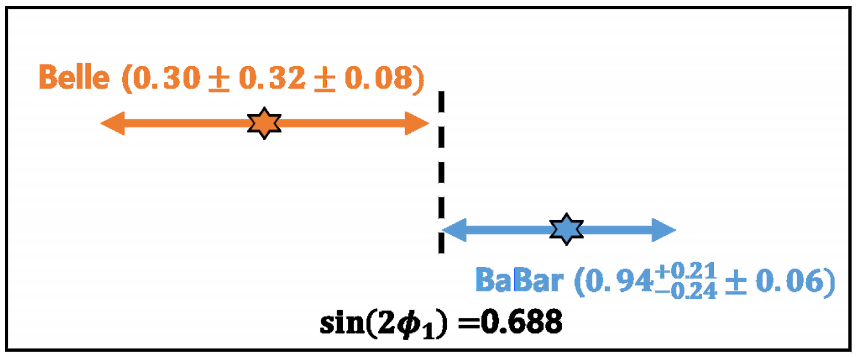
\includegraphics[height=5cm]{belle_babar_result}
\caption{The results of Belle (2007) and Babar on -sin(2$\phi_1$)}
\end{figure}
\end{comment}


\section{Data Sample and Event Selection}
\begin{comment}
The simulation data (MC) is taken from Belle II official MC campaign 13, named MC13. Both signal MC and generic MC are produced. In signal MC, one of the $B^0$ from $\Upsilon(4S)$ decays into final states 3$K_S^0$ then into 6 charged pions, while the other $B^0$ decays generically using all possible channels. In generic MC,  $B^0$ from  $\Upsilon(4S)$ all decay generically using all possible channels.
The signal MC sample is produced by EvtGen package with provided ``decay.dec" file that describes the required decay mode and branching fraction. As $K_S^0 \to \pi^0 \pi^0$ leads to large background with poor vertex quality, only the final states to 6 charged pions is used.
\end{comment}

As introduced in section 2.9, the branching fraction of $\mathcal{B}(B^0 \to K_S^0  K_S^0  K_S^0) = 6.0 \times 10^{-6}$. The simulation takes the $\Upsilon(4S)$ as the mother particle and generate its decay process to two scalar $B^0$ mesons with mixing. $B^0 \to K_S^0  K_S^0  K_S^0$ is simulated based on only the possible phase-space of kinematics that final states could have, which no $\it{CP}$ violation is assigned for $\mathcal{S}$(sin2$\phi_1$) and $\mathcal{A}$ in both signal and generic MC.

\subsection{$K_S^0$ Selection}
$K_S^0$ reconstruction is first reconstructed by the cut-based reconstruction which contains a large fraction of fake candidates, as discussed in chapter 3. In addition, a momentum cut on $K_S^0$ is used considering distribution in $B^0 \to K_S^0  K_S^0  K_S^0$. Only the $K_S^0$ candidates with momentum larger than 0.05 GeV are selected, as shown in Figure \ref{fig:ks-p}. 
\begin{figure}[ht]
	\centering
	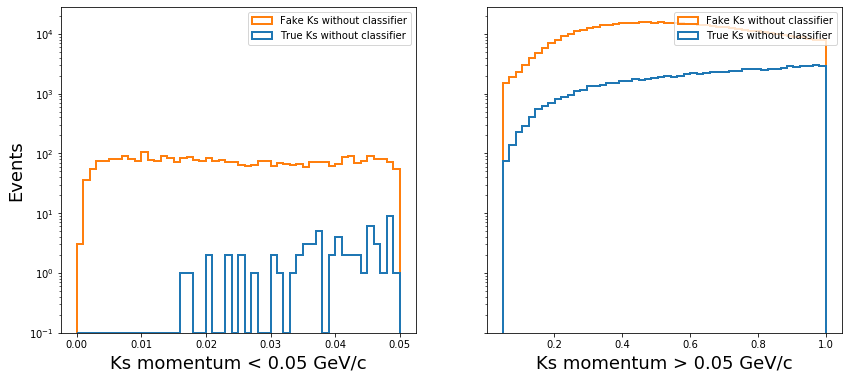
\includegraphics[height=6.5cm]{ks-p}
	\caption{The distribution of $K_S^0$ momentum. Candidates smaller than 0.05GeV/c are rejected. (Both plots shares the same y-axis scale on the left side.)}
	\label{fig:ks-p}
\end{figure}
Next, the vertex fit of $K_S^0$ is performed using \textit{TreeFit} package\cite{refId0}. Using fitted $K_S^0$ momentum and energy, fitted invariant mass is different from the one obtained directly using daughters' 4-vector. This quantity often receives impact of the measurement uncertainties. If we check out the distribution of fitted invariant mass based on daughters' SVD hits as section 3.1 discussed, \textit{SVD00} $K_S^0$ shows a large dispersion from the central region of the distribution of invariant mass after vertex fit, while \textit{SVD11} $K_S^0$ shows a small dispersion as shown in Figure \ref{fig:invm1}. Therefore, considering the $K_S^0$ candidates with different SVD hits, see Figure \ref{fig:ks-r-svdxx} and Table \ref{tab:svdxx}, reflecting the different tracking quality of daughter $\pi^{\pm}$, the different cut on invariant mass M$_{\pi^+\pi^-}$ after vertex fit is applied depending on the SVD hits number of pion tracks. As shown in Figure \ref{fig:invm}, the sideband regions where fake $K_S^0$ is much higher than true $K_S^0$ are excluded. The cut windows are listed in Table \ref{tab:ks_invm}. This improves the reconstruction purity.

\begin{figure}[htpb]
\centering
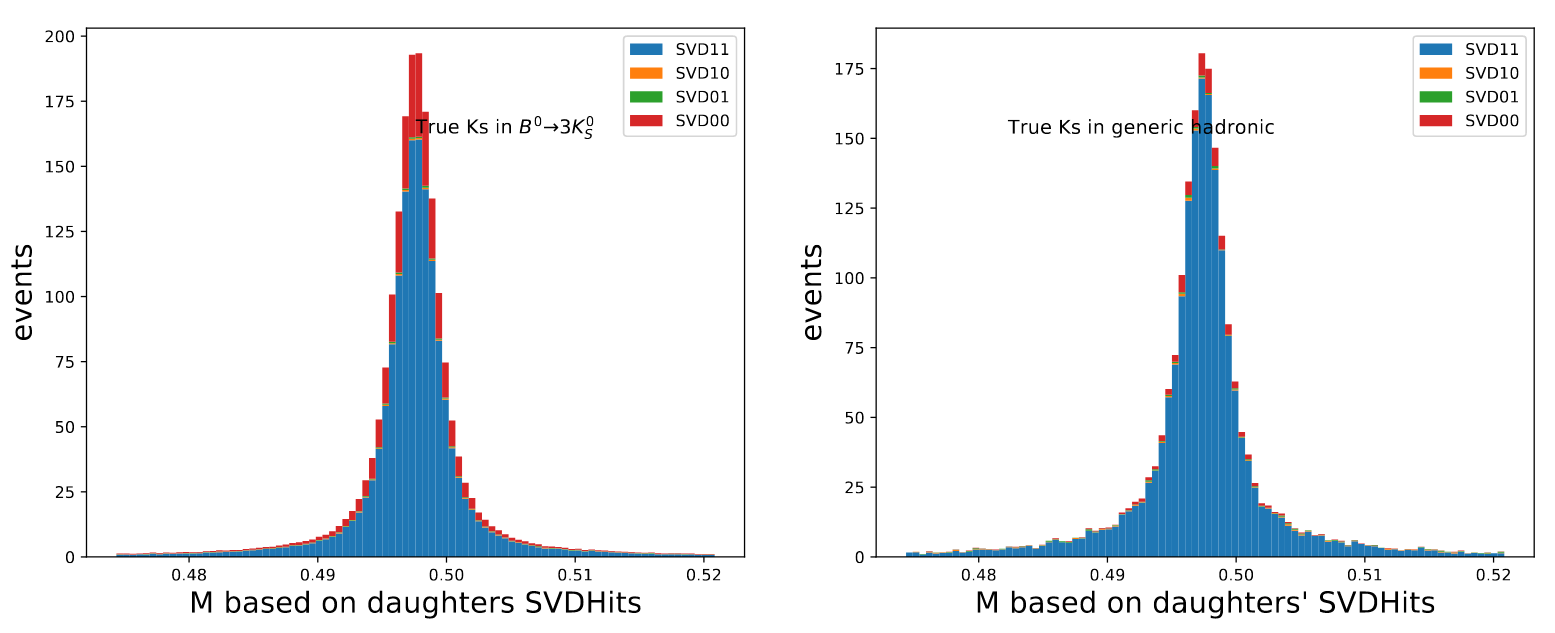
\includegraphics[width=0.7\linewidth]{m-before-fit}
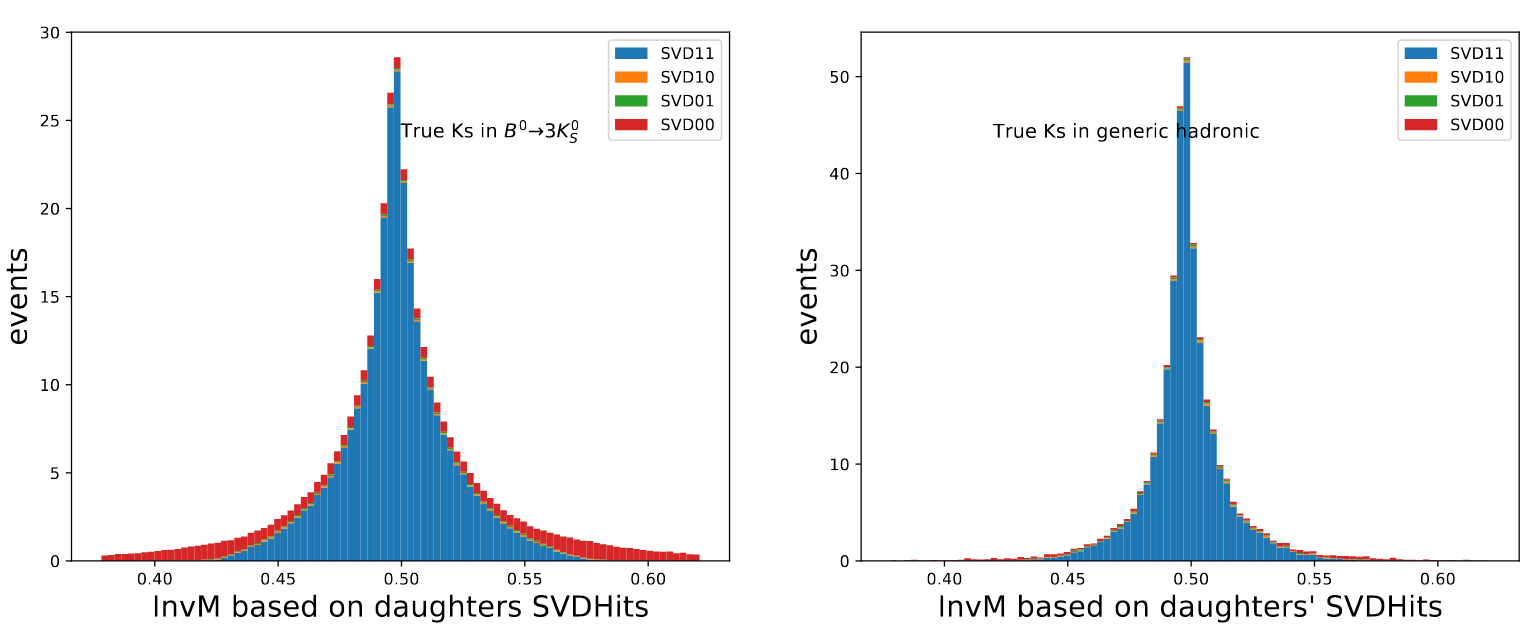
\includegraphics[width=0.7\linewidth]{m-after-fit}
\caption{(Top two plots)The invariant mass from daughters' 4-vector, the left is $B^0 \to K_S^0  K_S^0  K_S^0$  signal MC and the right is generic MC;
(bottom two plots)The invariant mass after vertex fit, the left is $B^0 \to K_S^0  K_S^0  K_S^0$  signal MC and the right is generic MC;
In both cases, the red shows the clear dispersion on \textit{SVD00} type $K_S^0$.}
\label{fig:invm1}
\end{figure}
 
In summary, $K_S^0$ are first reconstructed using BASF2 standard library with all converged vertex fit candidates are kept using \textit{TreeFit}. Then we reject $K_S^0$ candidates with momentum smaller than 0.05 GeV/c. After this, tuned cuts on invariant mass after vertex fit for each $K_S^0$ based on their SVD hits of pions are applied according to Table \ref{tab:ks_invm}. 
Eventually, only $K_S^0$ with ``FBDT\_Ks" larger than 0.74 are kept based on Figure \ref{fig:ks_fom}.
 
\begin{table}[h]
	\centering 
	\begin{tabular}{|c|c|c|c|c|} 
		\hline
		$K_S^0$ type & SVD11 & SVD10 & SVD01  & SVD00  \\
		\hline
		M$_{\pi^+\pi^-}$ window (GeV) & (0.45,0.55) & (0.38,0.7)  & (0.38,0.7)  & (0.3,0.7) \\
		\hline
	\end{tabular}
\caption{Invariant mass cut window after vertex fit for $K_S^0$ based on Figure \ref{fig:invm}.}
\label{tab:ks_invm}
\end{table}

\begin{figure}[htpb]
	\centering
	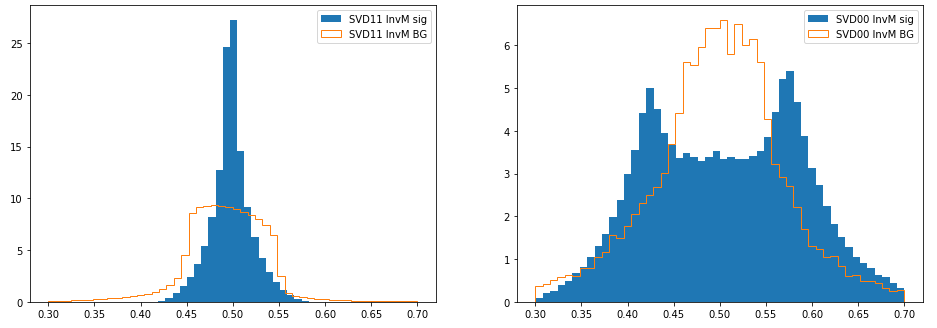
\includegraphics[width=0.7\linewidth]{invm1}
	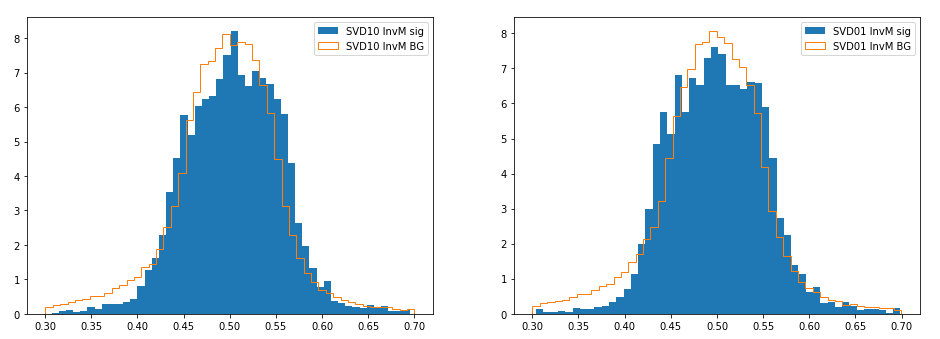
\includegraphics[width=0.7\linewidth]{invm2}
	\caption{Invariant mass after vertex fit of $K_S^0$, the sideband is excluded in each distribution to further reject fake $K_S^0$}
	\label{fig:invm}
\end{figure}

\subsection{$B^0$  Reconstruction}

By combining three $K_S^0$ particles from selected dataset, we can reconstruct $B^0$. The beam-constraint mass $M_{bc}$ and energy difference $\Delta E$ are used to extract signal, as defined in Equation \ref{eq:mbc} and \ref{eq:dE}, respectively. For $M_{bc}$, $s$ is defined as the invariant mass and $p^*_B$ is the reconstructed $B$ momentum, both in the center-of-mass frame of $e^+e^-$. For $\Delta E$, $E^*_B$ is the reconstructed energy in the center-of-mass frame of $e^+e^-$. These two variables are quite useful for discriminating signal and background events for hadronic $B$ decay with fully reconstructed final states.
 In Belle II, the $B^0$ candidates with $M_{bc} > 5.2$ GeV and $|\Delta{E}| < 0.2$ GeV are requested to be reconstructed. The $B^0$ vertex fit using \textit{TreeFit} is performed on each $B^0$ candidate and only $B^0$ with converged vertex fit result is kept (by a very loose cut of "$\text{chiProb} > 0.001$" ), which is essential to obtain the decay vertex positions of $B$ mesons for further $\it{CP}$ violation analysis. When multiple $B^0$ candidates are obtained in a single event, the best candidates selection (BCS) is performed by ranking their vertex fit quality. Since the BCS is based on the vertexing quality that might introduce bias in the vertex positions for $\it{CP}$ fit, we check the distribution of the vertex $\chi_2$, as shown in Figure \ref{fig:b0dist} top right where the data and generic MC present a good consistence within $1\sigma$ on average. The distribution of candidates number per event without BCS is shown in top left of Figure \ref{fig:b0dist} as well, showing an agreement between data and generic MC within 1$\sigma$. The distribution of candidates per event is also in an agreement with that from signal MC (bottom left of Figure \ref{fig:b0dist}). The 2D distribution of $M_{bc}$ and $\Delta E$ from $B^0 \to K_S^0  K_S^0  K_S^0$ signal MC is shown in Figure \ref{fig:b0dist}  bottom right, where the correlation factor is about 15\% between two observables. 
 \begin{equation}\label{eq:mbc}
 M_{bc} = \sqrt{\frac{s}{4}-p^{*2}_B} 
 \end{equation}
 \begin{equation}\label{eq:dE}
 \Delta E = E^*_B - \frac{\sqrt{s}}{2}
 \end{equation}
 
\begin{figure}[H]
	\begin{minipage}[b]{0.5\linewidth}
		\centering 
		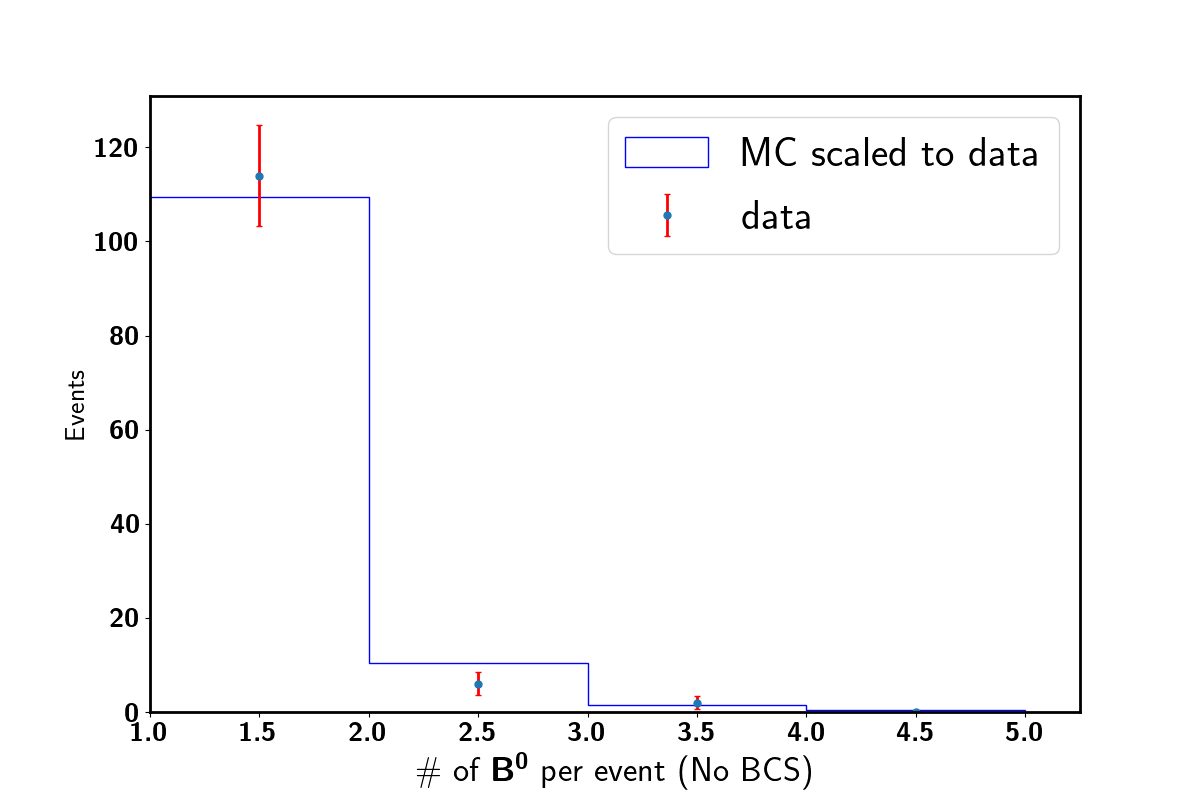
\includegraphics[height=6cm]{figures/best_ncands_noBCS}
		
	\end{minipage}
	\begin{minipage}[b]{0.5\linewidth}
		\centering 
		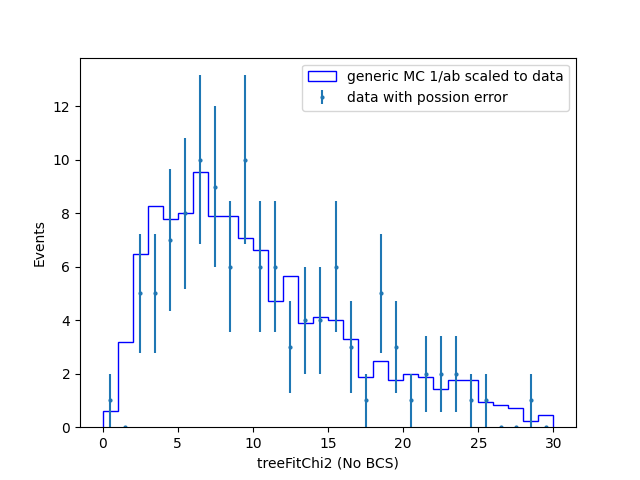
\includegraphics[height=6cm]{figures/best_treeFitChi2_noBCS}
		
	\end{minipage}
	\begin{minipage}[b]{0.5\linewidth}
		\centering 
		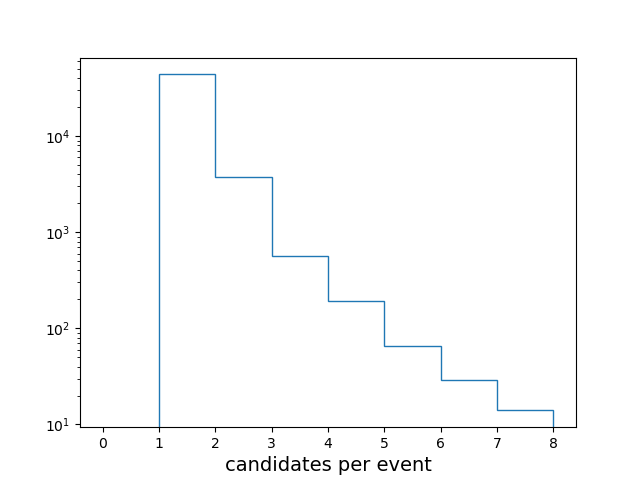
\includegraphics[height=6cm]{figures/best_cands}
		
	\end{minipage}
	\begin{minipage}[b]{0.5\linewidth}
		\centering 
		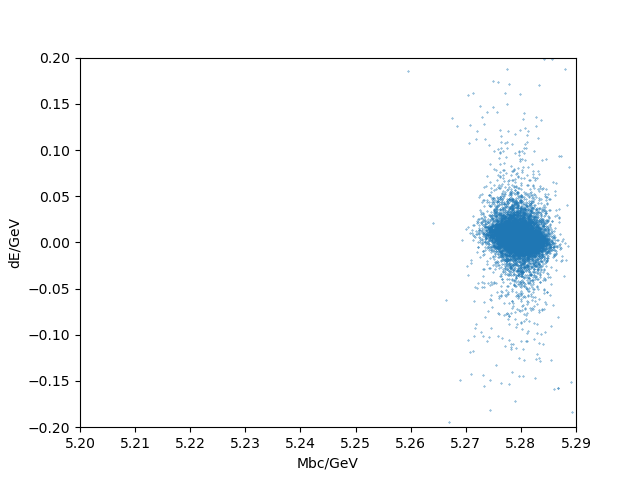
\includegraphics[height=6cm]{figures/hist_sig_MC_Mbc_dE}
		
	\end{minipage}
	
	\caption{Top left is the candidates per event in data and generic MC before the BCS. Top Right is the $\chi_2$ for data and generic MC before BCS. Bottom left is the number of candidates $B^0$ per event from signal MC. Bottom right is the 2D $M_{bc}$ and $\Delta E$ distribution from signal MC.}
	\label{fig:b0dist}
\end{figure}

% move to after CS
\subsection{Continuum Suppression}
The production cross-section of $B\bar{B}$ from $\Upsilon{(4S)}$ receives a sizable contribution from other flavor of quarks other than b quark. This calls a demand to distinguish a specific $B\bar{B}$ decay events from combinatorial background from $e^+e^- \to q\bar{q}$, so called continuum suppression (CS). The rejection is essential because it's the dominated background.  In the case of $b \to s$ charmless decay like $B^0 \to K_S^0  K_S^0  K_S^0$, the number of continuum background can exceed the signals by a few orders of magnitudes without suppression. In a $B\bar{B}$ event, two mesons are produced almost at rest in the CMS frame since the resonance state $\Upsilon(4S)$ is  just slightly lighter than beam energy. As a result	, decay products are emitted more isotopically, compared to continuum background. The ARGUS and CLEO collaboration\cite{Bevan_2014} developed a set of variables to suppress the continuum, which has also been implemented into BASF2 framework. 

CLEO cones momentum can be presented as Equation \ref{eq:ln}, where $ p_i $ is momentum of i-th particle in Rest-Of-Event (ROE) particles in a event except for the ones used to reconstructed $\it{CP}$-side $B^0$, $\theta_i$ is angle against momentum thrust of reconstructed $\it{CP}$-side of \textit{B} meson.

\begin{equation}\label{eq:ln}
L_n = \sum_{i\in ROE}^{} p_i \times |cos\theta_i|
\end{equation}

Besides, the modified Super Fox-wolfram momentum named  KSFW momentum, are calculated in each event. The KSFW momentum are defined as shown in Equation \ref{eq:ksfw}. 
\begin{equation}\label{eq:ksfw}
KSFW = \sum_{l=0}^{4}( R_l^{so} + R_l^{oo}) + \gamma \sum_{n=1}^{N_t}|P(t)_n|
\end{equation}
where the first term is shown in Equation \ref{eq:rlso}.
\begin{equation}\label{eq:rlso}
R_l^{so} = \frac{\alpha_{cl}H_{cl}^{so} +
				\alpha_{nl}H_{nl}^{so}+
			\alpha_{ml}H_{ml}^{so}}{E^*_{beam}-\Delta E}
\end{equation}

when l is odd in Equation \ref{eq:rlso}: 
\begin{equation}
	H_{nl}^{so}=H_{ml}^{so}=0
\end{equation}
and $H_{cl}^{SO}$ is defined as shown in Equation \ref{eq:hclso}: 
\begin{equation}\label{eq:hclso}
	H_{cl}^{so} = \sum_i \sum_{jx}Q_i Q_{jx}|p_{jx}|P_l(cos\theta_{i,jx})
\end{equation}
\textit{i} runs over \textit{B} daughter particles and \textit{jx} for other particles in ROE. \textit{Q} is charge and $p_{jx}$ is momentum for each particle. $P_l(cos\theta_{i,jx})$ is the \textit{i}-th order Legendre polynomial of cosine of \textit{i} and \textit{jx}-th particles.
On the other hand, for \textit{l} is even, $H_{xl}^{SO}$ can be written in Equation \ref{eq:hxlso}.
\begin{equation}\label{eq:hxlso}
	H_{xl}^{so}=\sum_i \sum_{jx}|p_{jx}|P_l(cos\theta_{i,jx})
\end{equation}
The second term in Equation \ref{eq:ksfw}, when \textit{l} is odd, can be defined as Equation \ref{eq:roo}.
\begin{equation}\label{eq:roo}
	R^{oo}_l = \sum_j \sum_k \beta_l Q_j Q_k |p_j||p_k|P_l(cos\theta_j,k)
\end{equation}
\textit{j} and \textit{k} runs over ROE particles and others are same as Equation \ref{eq:hclso}.
For an even \textit{l}: 
\begin{equation}
	R^{oo}_l = \sum_j \sum_k \beta_l |p_j||p_k|P_l(cos\theta_j,k)
\end{equation}
$\beta$ is Fisher coefficients to be determined. 
Using above definitions, we can form the possibility density functions for KSFW, cosine angle against \textit{B} meson thrust cos$\theta_B$ and $\Delta Z$ of two side vertices.  Then based on each event's variables' value, we can calculate a ratio $\mathcal{R}$ as Equation \ref{eq:Rcs}, where the likelihood $L$ of signal($L_S$) and background($L_B$) are obtained from the possibility density functions defined in Equation \ref{eq:Lsb}.
The $ \mathcal{R} $ is: 
\begin{equation}\label{eq:Rcs}
	\mathcal{R} = \frac{L_S}{L_S+L_B}
\end{equation}
\begin{equation}\label{eq:Lsb}
L_{S/B} = P(KSFW)_{S/B} \times P(cos\theta_B)_{S/B} \times P(\Delta Z)_{S/B}
\end{equation}
where \textit{P} is probability density function for signal and continuum, depending on the discriminating variables in the parentheses. For example, the distribution of a variable called $R_2$ shown in Figure \ref{fig:R2} where the possibility density function is different for signal and continuum events in generic MC.

\begin{figure}[H]
	\centering
	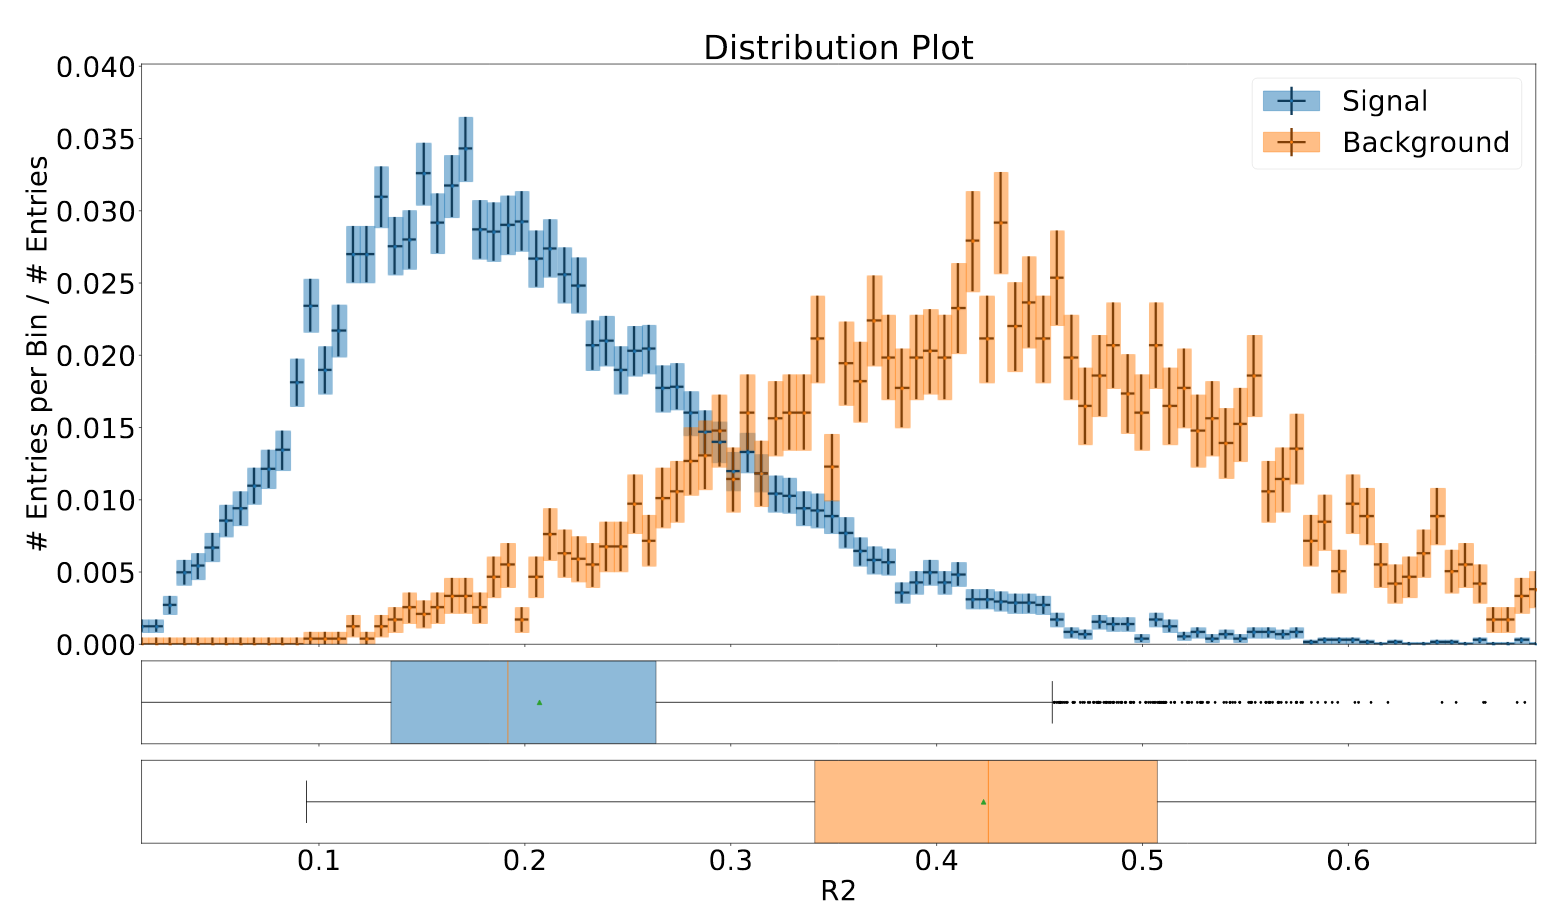
\includegraphics[width=0.7\linewidth]{r2}
	\caption{$R_2$ is the ratio of the second to the zeroth KSFW momentum in Equation \ref{eq:ksfw}. Its distribution in generic MC sample which serves as the highest weight as a variable in discriminating the continuum events, having a quite different distribution between signal and background.}
	\label{fig:R2}
\end{figure}



  In order to maximize suppression power in this analysis, these variables (KSFW, CLEO cone momentum and angular distributions) are combined as an input for FastBDT classifier. The targeted variable is the continuum event truth. The MC samples using signal $B\bar{B}$ events from signal MC and continuum events from generic MC ($q\bar{q}$ component) are prepared in a ratio of their cross-section at $\Upsilon{(4S)}$ energy. The same events reconstruction procedures for $B^0$ is applied for both MC samples. Events passing the reconstruction for $B^0$ using $M_{bc}$ and $\Delta E$ are used for training the continuum suppression classifier. The fraction of signal and background is set to 1:1 during the training.  The output of continuum suppression classifier is renamed as ``FBDT\_CS". Then we determine the cut value at 0.66 based on the maximum of \textit{FOM} curve, as shown in Figure \ref{fig:cs_fom}. The variables used in training are listed in Table \ref{tab:cs_abr} with their abbreviations and the rank of important variables is in Table \ref{tab:cs_imp}.

The correlation between these training variables are shown in Figure \ref{fig:cs_cor}. The correlation among the variables are varied in signal and background. The ROC curve and the efficiency/purity with respect to the classifier output are shown in Figure \ref{fig:cs_roc}.
\begin{table}[htpb]
	\begin{minipage}[t]{0.4\linewidth}
		\centering
		\caption{Variables and the abbreviations for CS.}
		\label{tab:cs_abr}
		\begin{tabular}{c|c}
			\hline
			Observables &  Abbreviations\\
			\hline
			CleoConeCS(9,) &  CleoC1 \\
			KSFWVariables(hoo1,) & KSFWV1 \\
			CleoConeCS(7,) & CleoC2\\
			CleoConeCS(5,) & CleoC3\\
			KSFWVariables(hso22,) & KSFWV2\\
			KSFWVariables(hoo3,) & KSFWV3\\
			CleoConeCS(4,) & CleoC4 \\
			KSFWVariables(hoo4,) &  KSFWV4\\
			CleoConeCS(3,) & CleoC5 \\
			CleoConeCS(6,) & CleoC6\\
			CleoConeCS(8,) & CleoC7\\
			KSFWVariables(hso14,) &   KSFWV5\\
			KSFWVariables(hso00,) & KSFWV6\\
			KSFWVariables(et,) & KSFWV7\\
			KSFWVariables(hso24,) & KSFWV8\\
			KSFWVariables(hso04,) & KSFWV9\\
			KSFWVariables(hso20,) & KSFWV10 \\
			KSFWVariables(mm2,)  & KSFWV11\\
			KSFWVariables(hoo2,) &  KSFWV12\\
			thrustOm & thrus1 \\
			cosTBz & cosTB1\\
			CleoConeCS(1,) & CleoC8 \\
			CleoConeCS(2,) & CleoC9 \\
			KSFWVariables(hso02,) &  KSFWV13\\
			KSFWVariables(hoo0,) &  KSFWV14 \\
			KSFWVariables(hso12,) &  KSFWV15\\
			KSFWVariables(hso10,) & KSFWV16\\
			cosTBTO & cosTB2\\
			thrustBm & thrus2\\
			R2 & R2\\
			\hline
		\end{tabular}
	\end{minipage}
	\begin{minipage}[t]{0.5\linewidth}
		\centering 
		\caption{The rank of important variables for CS. }
		\label{tab:cs_imp}
		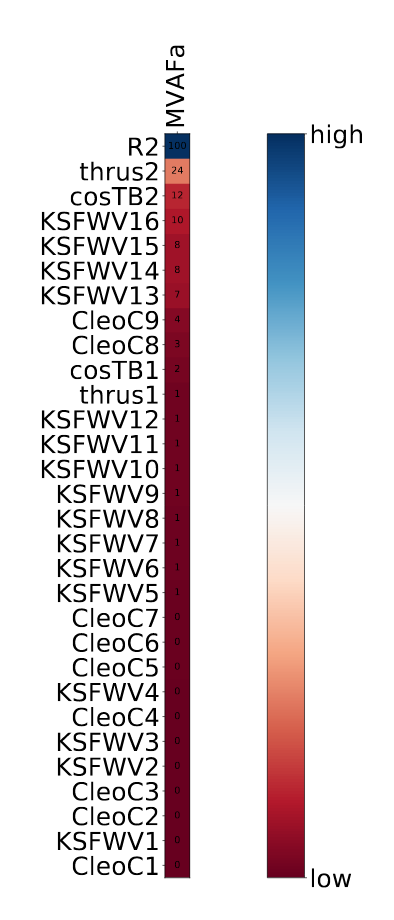
\includegraphics[width=4cm]{cs-imp}
	\end{minipage}
\end{table}

\begin{figure}[ht]
	\begin{minipage}[b]{0.5\linewidth}
		\centering 
		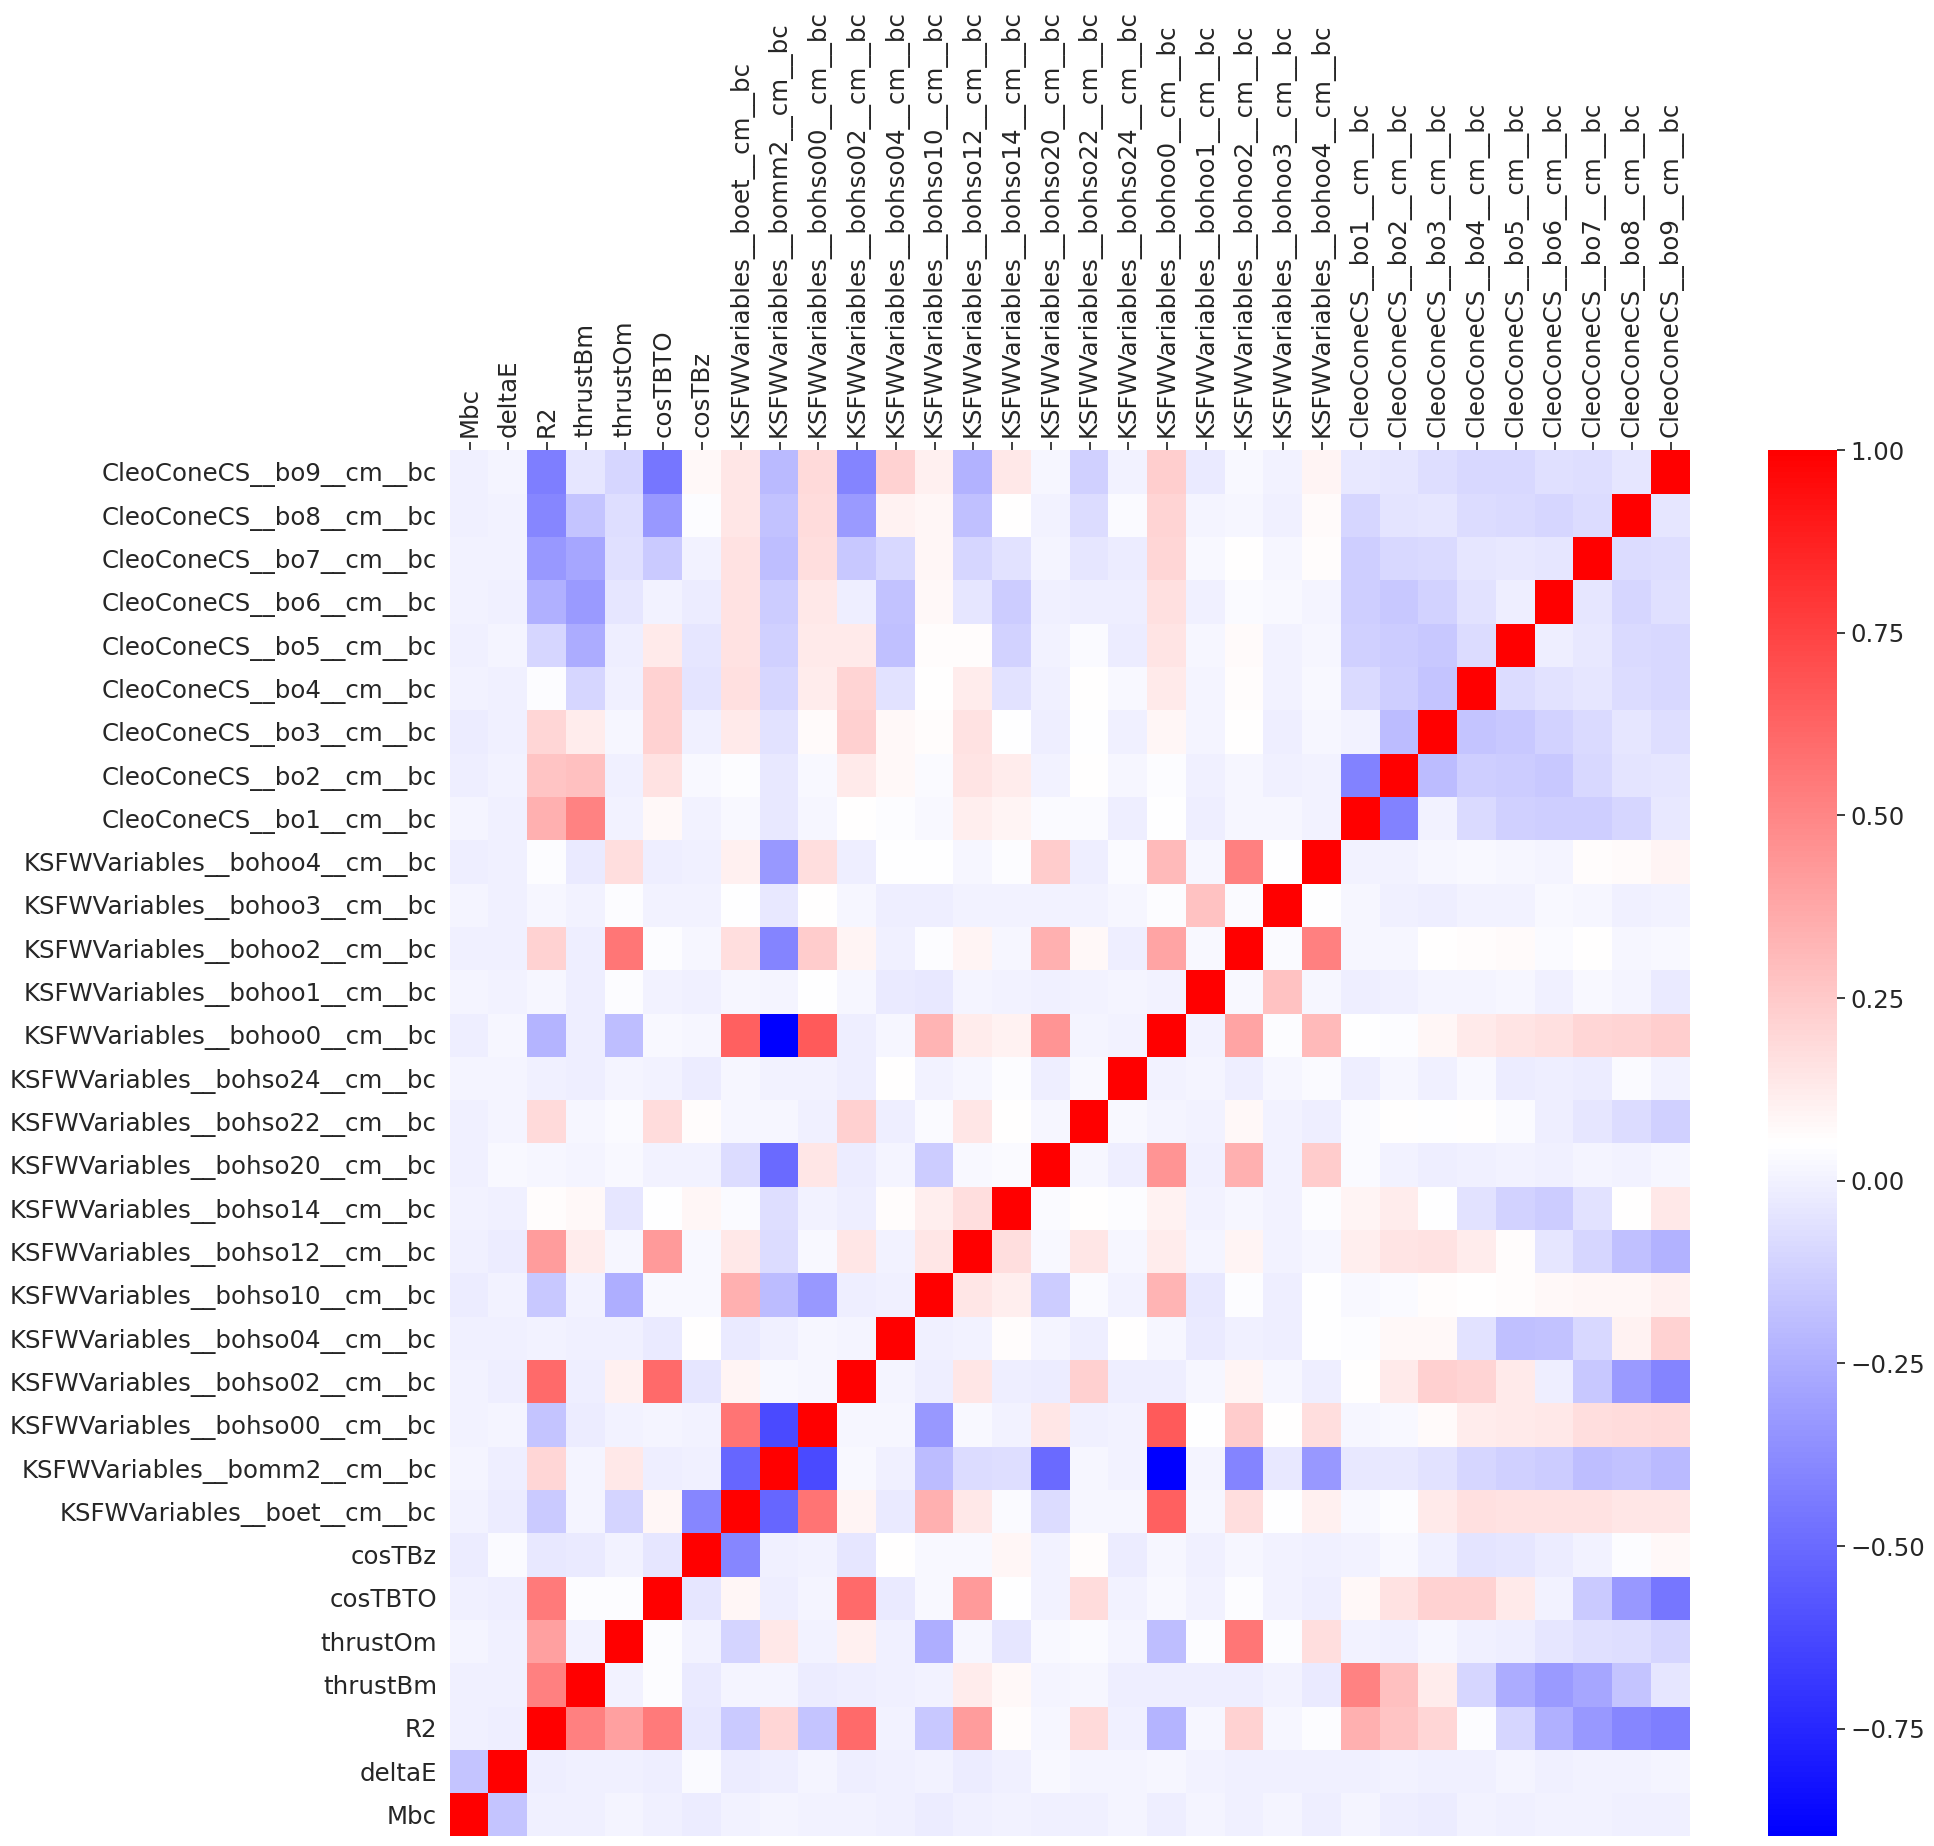
\includegraphics[height=7cm]{figures/corr_cs_kine_sig}	
	\end{minipage}
\begin{minipage}[b]{0.5\linewidth}
	\centering 
	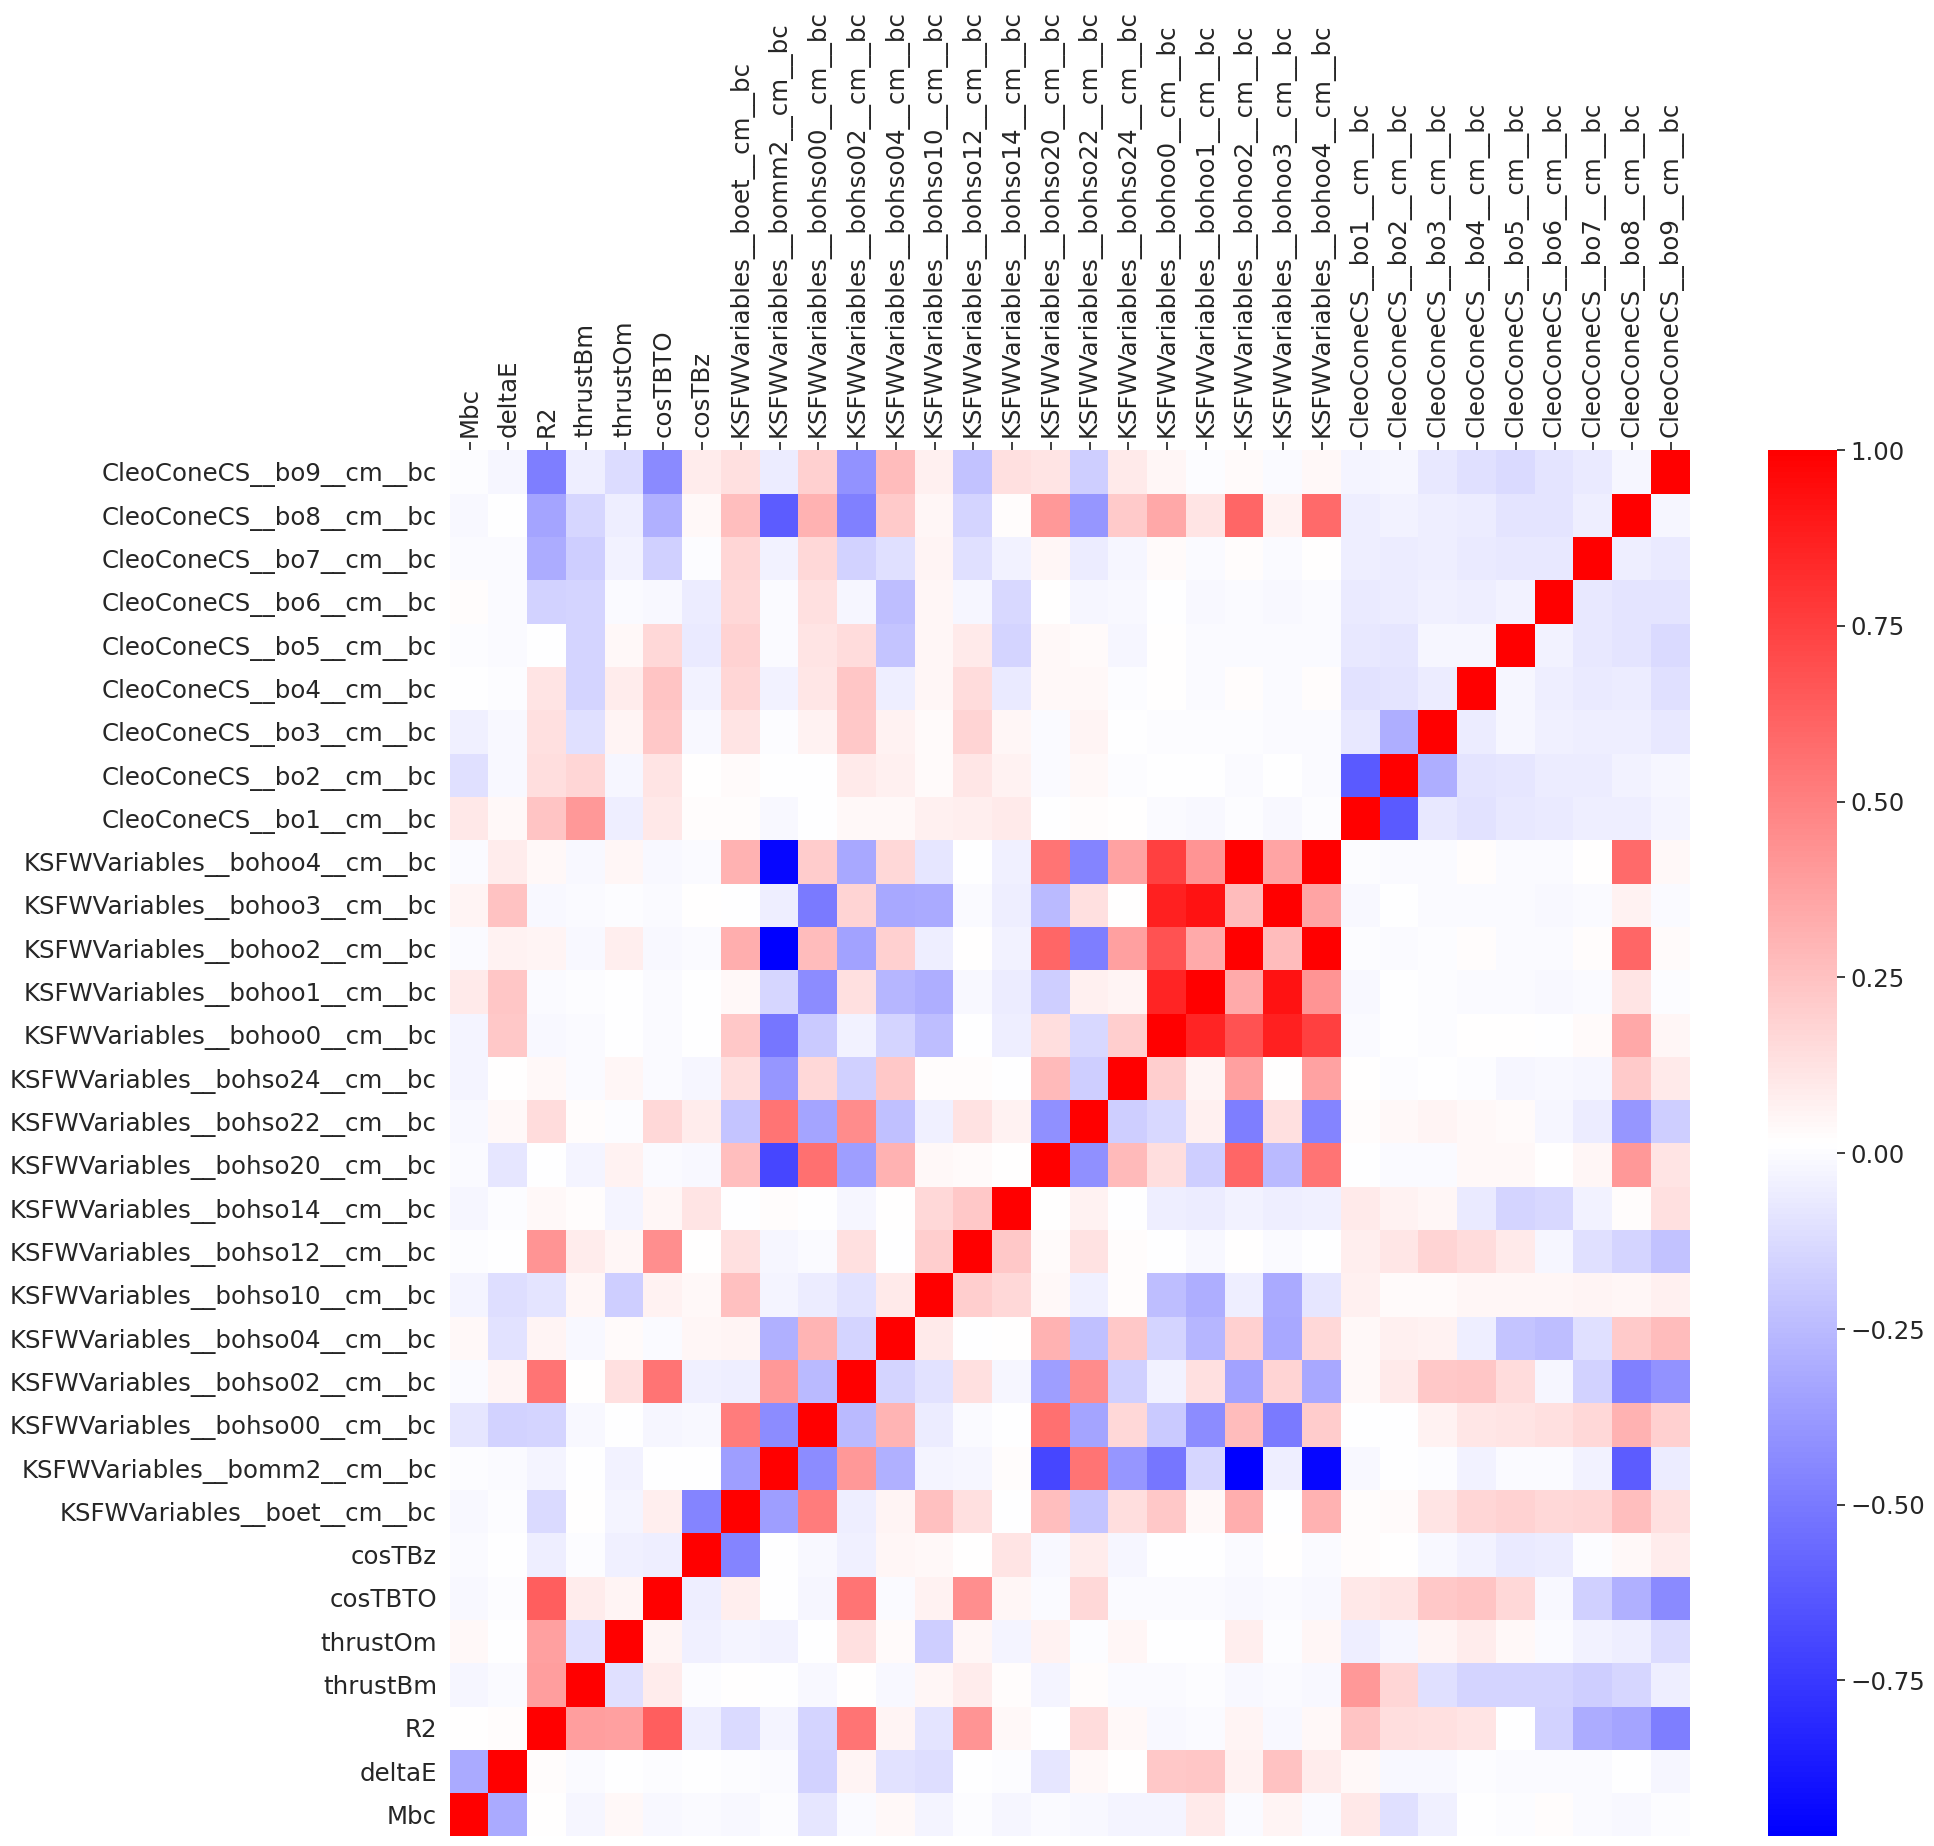
\includegraphics[height=7cm]{figures/corr_cs_kine_bkg}	
\end{minipage}
	\caption{The correlation in variables for continuum suppression. The left is for signal and the right is for background.}
	\label{fig:cs_cor}
\end{figure}
\begin{figure}[ht]
	\begin{minipage}[b]{0.5\linewidth}
		\centering 
		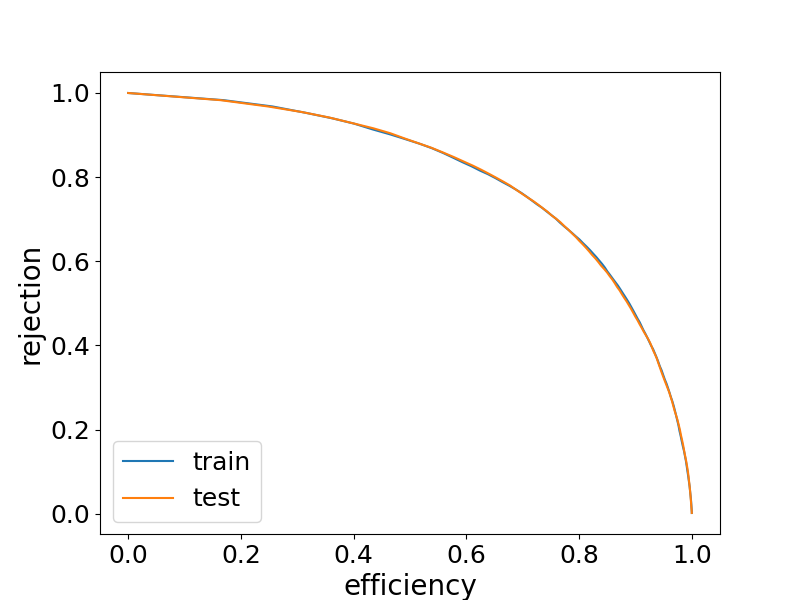
\includegraphics[height=5cm]{figures/ROC_CS}	
	\end{minipage}
	\begin{minipage}[b]{0.5\linewidth}
		\centering 
		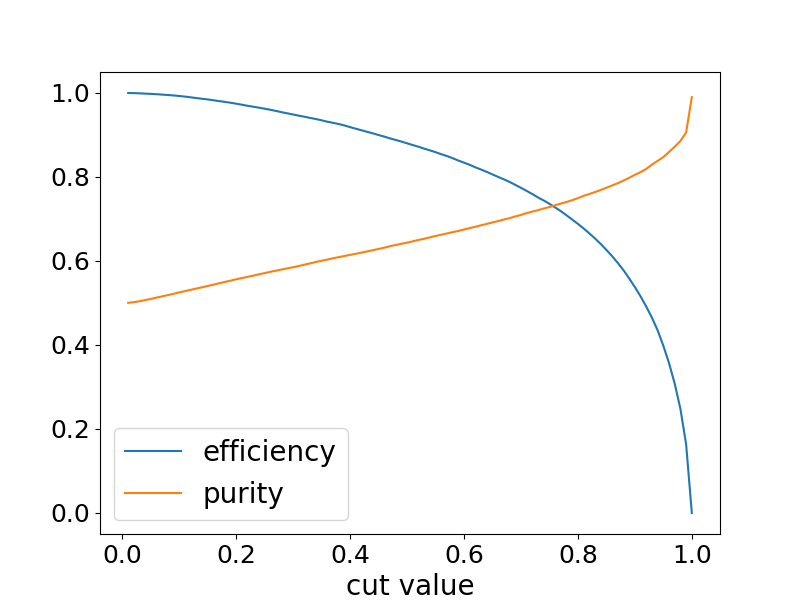
\includegraphics[height=5cm]{figures/eff_CS}	
	\end{minipage}
\caption{The left is the ROC curve (blue for training and orange for testing)
	and the right is the efficiency(blue) and purity(orange) regarding the classifier output ``FBDT\_CS"}
	\label{fig:cs_roc}
\end{figure}
Overtraining check is made by comparing the distribution of signal and background depending on the classifier output in both training and testing samples. The testing samples show about 1\% lower in each bin for both signal and background events, which is within the acceptable range.  
\begin{figure}[H]
	\centering
	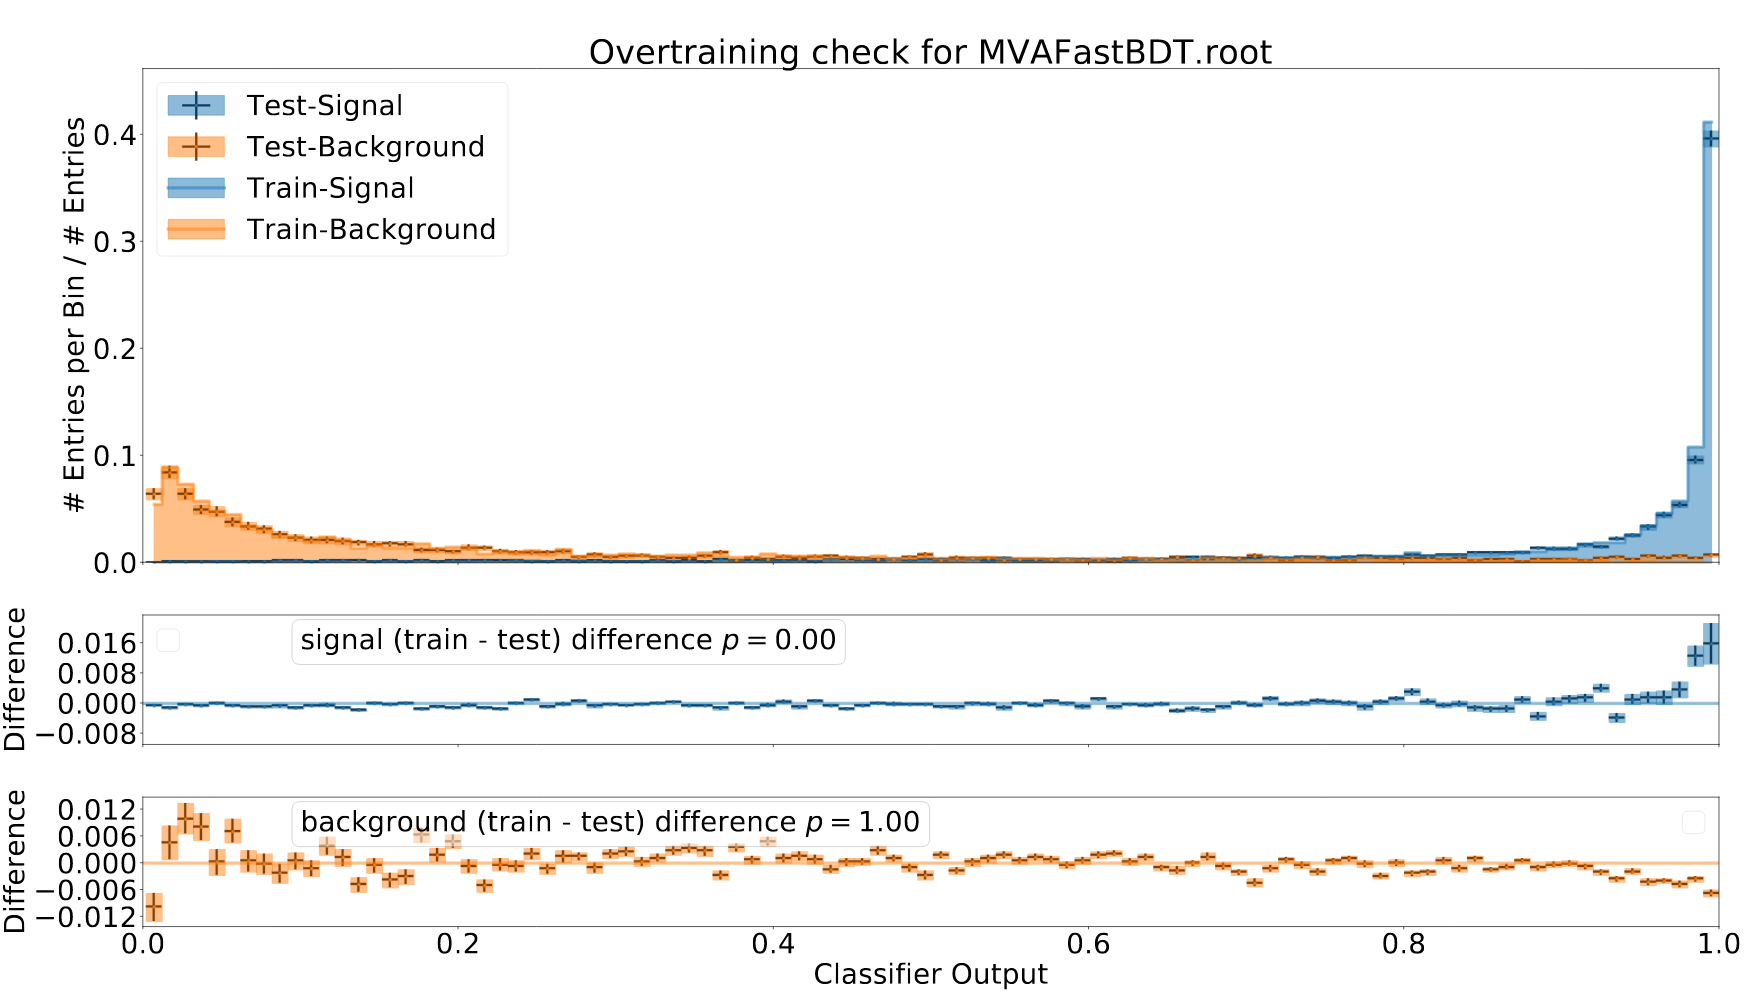
\includegraphics[width=0.8\linewidth]{cs-overtrain}
	\caption{Over-training check of continuum classifier, where a very small difference in training and testing (1\%) is shown.}
\end{figure}

\begin{figure}[H]
	\centering
	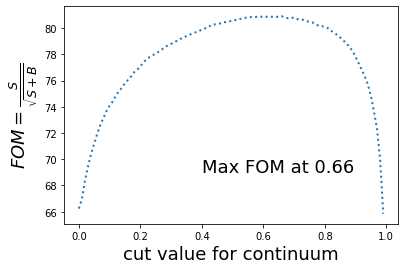
\includegraphics[width=0.6\linewidth]{cs-fom}
	\caption{\textit{FOM} depending on the cut value of continuum classifier output, cut value at 0.66 is used for continuum suppression. }
	\label{fig:cs_fom}
\end{figure}

The summary of $B^0$ selections is listed in Table \ref{tab:b0select}, including the application of KsFinder (by ``FBDT\_Ks") and continuum suppression (by ``FBDT\_CS").
\begin{table}[H]
	\centering 
	\begin{tabular}{|c|c|c|c|c|c|c|c|} 
		\hline
		$B^0$  & $M_{bc}$/GeV& $\Delta E$/GeV & chiProb & Rank & FBDT\_CS & FBDT\_Ks\\
		\hline
		Selection & $> 5.20$ \& $< 5.29$  &  $ |\Delta E|< 0.2$ & $> 0.001$  & $=1$ & $>0.66$ & $>0.74$\\
		\hline
	\end{tabular}
	\caption{$B^0$ selection criteria, ``chiProb" is from $B^0$ vertex fit and ``Rank" is from best candidate selection.}
	\label{tab:b0select}
\end{table}

Explicitly, the reconstruction performance of $B^0$ is summarized in Table \ref{tab:b0stats}, the efficiency, purity, fraction of multiplicity events and best candidates fraction of $B^0$ is slight improved in Belle II compared to Belle.
\begin{table}[H]
	\centering
	\begin{tabular}{c|c|c|c|c}
		\hline
		event selection & efficiency & purity  & $f_{MB}$  & BCS \\
		\hline
		\hline
		Belle Standard & 35\%(33\%) & 96\%(99\%) & 6\%(6\%) & 83\%(96\%)\\
		\hline 
		Belle II (BG1) & 36\%(34\%) & 96\%(98\%) & (4\%)(4\%) & 95\%(96\%)\\
		\hline
		Belle II (BG0) & 40\%(36\%) & 96\%(99\%) & (3\%)(3\%) & 97\%(97\%)\\
		\hline
	\end{tabular}
	\caption{The efficiency is defined by the fraction of best candidates among the MC input number. Purity is the fraction of true $B^0$ in best candidates. $f_{MB}$ stands for multiple $B^0$ events fraction in true signal events. BCS is the fraction of best candidates being a true signal. All values in the parenthesis are calculated in $| M_{bc} |- 5.28 < 0.1$ and $|\Delta E| < 0.1$, called as ``signal region" where efficiency is lower but purity is higher, compared to the full range of $M_{bc}$ and $\Delta E$ in Table \ref{tab:b0select}. }
	\label{tab:b0stats}
\end{table}


% summary of $B^0$ stats goes here
\subsection{Resonance Background}
Besides the major contribution from continuum background, charmonium resonance that mediates through $b \to c$ transition brings odd $\textit{CP}$ eigenvalue in the final states as same as $B^0 \to K_S^0  K_S^0  K_S^0$. Monitoring their contribution is also important. Basically, one needs to check the resonance states formed by two $K_S^0$ with corresponding invariant mass. In $B^0 \to X(K_S^0 K_S^0) K_S^0$,  there are two types of resonant events that give out same final states, one is resonant signal and the other is resonant background. For $b \to s$ transitions as resonance signal because of the $\it{CP}$-even final states, \textit{X} could be $f_2(1270)$, $f_0(1500)$, $f_{2}^{'}(1525)$, $f_0(980)$, $f_0(1710)$ and $f_2(2010)$. For $b \to c$ transition as resonance background because of $\it{CP}$-odd final states, \textit{X} could be $D^0$, $J/\psi$, $\psi(2S)$,  $\chi_{c0}$, $\chi_{c1}$, and $\chi_{c2}$.

The number of these background in signal reconstruction could be further reduced by implementing veto on invariant mass of 2$K_S^0$. However, such veto should be carefully validated with data. The distribution of invariant mass of \textit{X} should agree well in MC and data, which is hard to check in the low luminosity. The distribution of 2$K_S^0$ invariant mass in generic MC and data are shown in the Appendix 


 Some of these resonance have not been implemented inside generic MC production in the current Belle II simulation. Given the very limited statistics of data accumulation we used in this analysis, we only present the expected number of these resonances in 400$fb^{-1}$ luminosity (about $2.14 \times 10^8$ events) from generic $\Upsilon{(4S)}$ events. These numbers should be re-checked in the future when data accumulation increases, and veto must be based on the structure of 2$K_S^0$ invariant mass from data as well. Details about the expected yields can be found in Table \ref{tab:f_res}. Currently there is no veto applied for rejecting these resonant background considering the estimated background number is about 1 event in the current luminosity.
\begin{sidewaystable}
	\caption{Expected yield for signal and background resonances $2.14\times 10^8 B\bar{B}$ in generic MC. The branching fraction of $B\to X K_S$ and $X \to 2K_S$ are listed for both PDG value and value in Belle II generic decay profile ()see section 2.9). The events from $\it{CP}$-odd contamination is expected to be very low at current luminosity (62.8 fb$^{-1}$).}
	\label{tab:f_res}
	\centering
	\begin{tabular}{|c|c|c|c|c|c|c|}
		\hline
		Resonances & Br($B \to X K_S$)PDG  & Br($X \to2K_S$) & Br($B \to X K_S$)Dec. & Br($X \to2K_S$)Dec. & $B\bar{B}$ pairs & Expected yields \\
		\hline
		$D^0 K_S$ & $2.6 \times 10^{-5}$ & $1.7\times 10^{-4}$ & $2.6 \times 10^{-5}$ & $1.8\times 10^{-4}$ & $2.14\times 10^8$ & 0.134 \\
		\hline
		$\eta K_S$ & $3.45\times 10^{-4}$ & $<3.1\times 10^{-4}$ & $4\times 10^{-4}$ & No Value & $2.14\times 10^8$ & No Value  \\
		\hline
		$J/\psi K_S$ & $4.35\times 10^{-4}$ & $<1.4\times 10^{-8}$ & $4.35\times 10^{-4}$ & 0 & $2.14\times 10^8$ & 0 \\
		\hline
		$\psi(2S)K_S$ & $2.9\times 10^{-4}$ & $<4.6\times 10^{-6}$ & $2.9\times 10^{-4}$ & 0 & $2.14\times 10^8$ & 0 \\
		\hline
		$\chi_{c0}K_S$ & $7.3\times 10^{-5}$ & $3.16\times 10^{-3}$ & $7.35\times 10^{-5}$ & $3.1\times 10^{-3}$ & $2.14\times 10^8$ & 6.21 \\
		\hline
		$\chi_{c1}K_S$ & $1.96\times 10^{-4}$ & $6\times 10^{-5}$ & $1.96\times 10^{-4}$ & $1\times 10^{-5}$ & $2.14\times 10^8$ & 0.05 \\
		\hline
		$\chi_{c2}K_S$ & $7.5\times 10^{-6}$ & $2.6\times 10^{-4}$ & $7.5\times 10^{-6}$ & $5.5\times 10^{}-4$ & $2.14\times 10^8$ & 0.11 \\
		\hline
		$f_2(1270)K_S$ & $1.35\times 10^{-6}$ & $1.15\times 10^{-2}$ & $1.35\times 10^{-6}$ & $1.15\times 10^{-2}$ & $2.14\times 10^8$ & 0.42 \\
		\hline
		$f_{2}^{'}(1525)K_S$ & $1.5\times 10^{-7} $ & $2.22\times 10^{-2}$ & No value & 0.22 & $2.14\times 10^8$ & No Value \\
		\hline
		$f_2(2010)K_S$ & $5\times 10^{-7}$ & No Value  & No Value  & No Value  & $2.14\times 10^8$ & No Value \\
		\hline
		$f_0(980)K_S$ & $2.7\times 10^{-6}$ & No Value & $2.75\times 10^{-6}$ & No Value & $2.14\times 10^8$ & 43.3 \\
		\hline
		$f_0(1710)K_S$ & $5\times 10^{-7}$ & No Value  & No Value  & No Value  & $2.14\times 10^8$ & No Value \\
		\hline
		$f_0(1500)K_S$ & $6.5\times 10^{-5}$ & 0.022 & No Value & 0.022 & $2.14\times 10^8$ & No Value \\
		\hline
		Total  & - & - & - & - & - & $\simeq$50 \\
		\hline
	\end{tabular}
\end{sidewaystable}


% 2021.02.10 mid
\subsection{$B\bar{B}$ background and self-cross feed}
Another possible contribution of backgrounds are from $B\bar{B}$ events including the charged and the neutral particles. The estimated contributions of these types can be checked with charged $B\bar{B}$ samples and the mixed samples. For this channel, the number of the events is very limited. Self-cross feed backgrounds stands for the events from the signal-like events but the tag-side particle(s) is associated as a fake signal. The combined contributions from $B\bar{B}$ background and self-cross feed is about 3\% in the channel and therefore we don't perform special treatment on them.

\subsection{Signal Extraction}
The event selections defined in Table \ref{tab:b0select} is applied to signal MC, generic MC and experiment data for signal extraction. As introduced in chapter 2, the integral luminosity in generic MC is 1 ab$^{-1}$ and experiment data used in this analysis is about 62.8 fb$^{-1}$ from the latest official processing. 

The unbinned maximum likelihood fit using RooFit is performed to extract the signal. The 2D fit using both $M_{bc}$ and $\Delta{E}$ are done by taking the probability density function as shown in Equation \ref{eq:pmbcde}.
\begin{equation}\label{eq:pmbcde}
\mathcal{P}(M_{bc},\Delta{E}) = 
f_{sig}\times \mathcal{P}_{sig}^{M_{bc}}\times\mathcal{P}_{sig}^{\Delta{E}}
+ 
(1-f_{sig})\mathcal{P}_{bkg}^{M_{bc}}\times\mathcal{P}_{bkg}^{\Delta{E}}
\end{equation}
where $\mathcal{P}_{sig}^{M_{bc}}$ and $\mathcal{P}_{sig}^{\Delta{E}}$ are the single Gaussian and triple Gaussian functions. The $f_{sig}$ is fraction of signal events based on $M_{bc}$ and $\Delta E$. The $\mathcal{P}_{bkg}^{M_{bc}}$ is  primarily continuum events, and presented as Argus distribution as Equation \ref{eq:Argus} shows, with a preset mass threshold at $c = 5.29$ GeV. 
\begin{equation}\label{eq:Argus}
f(x;\chi,c)=\frac{\chi^3}{\sqrt{2\pi}\Psi(\chi)}\cdot
\frac{x}{c^2}\sqrt{1-\frac{x^2}{c^2}}\cdot
exp\begin{Bmatrix}
-\frac{1}{2}\chi^2(1-\frac{x^2}{c^2})
\end{Bmatrix}
\end{equation}
 $x$ is defined in $0<x<c$. $\chi$ and $c$ are parameters of the distribution, $\Psi(\chi)=\Phi(\chi)-\chi\phi(\chi)-\frac{1}{2}$ where $\Phi(\chi)$ and $\phi(\chi)$  cumulative distribution and probability density functions of the standard normal distribution, respectively. 
 
 The $\mathcal{P}_{bkg}^{\Delta{E}}$ is modeled by the first order Chebyshev polynomials. The shape parameters of signal events are determined by fitting to signal MC, and  then fixed as constants in fitting of Equation \ref{eq:pmbcde} on $M_{bc}$ and $\Delta E$ for generic MC and experiment data. Fitting results on signal MC are shown in Figure \ref{fig:mbcde1D}. 
 \begin{figure}[htbp]
 	\begin{minipage}[b]{0.5\linewidth}
 		\centering 
 		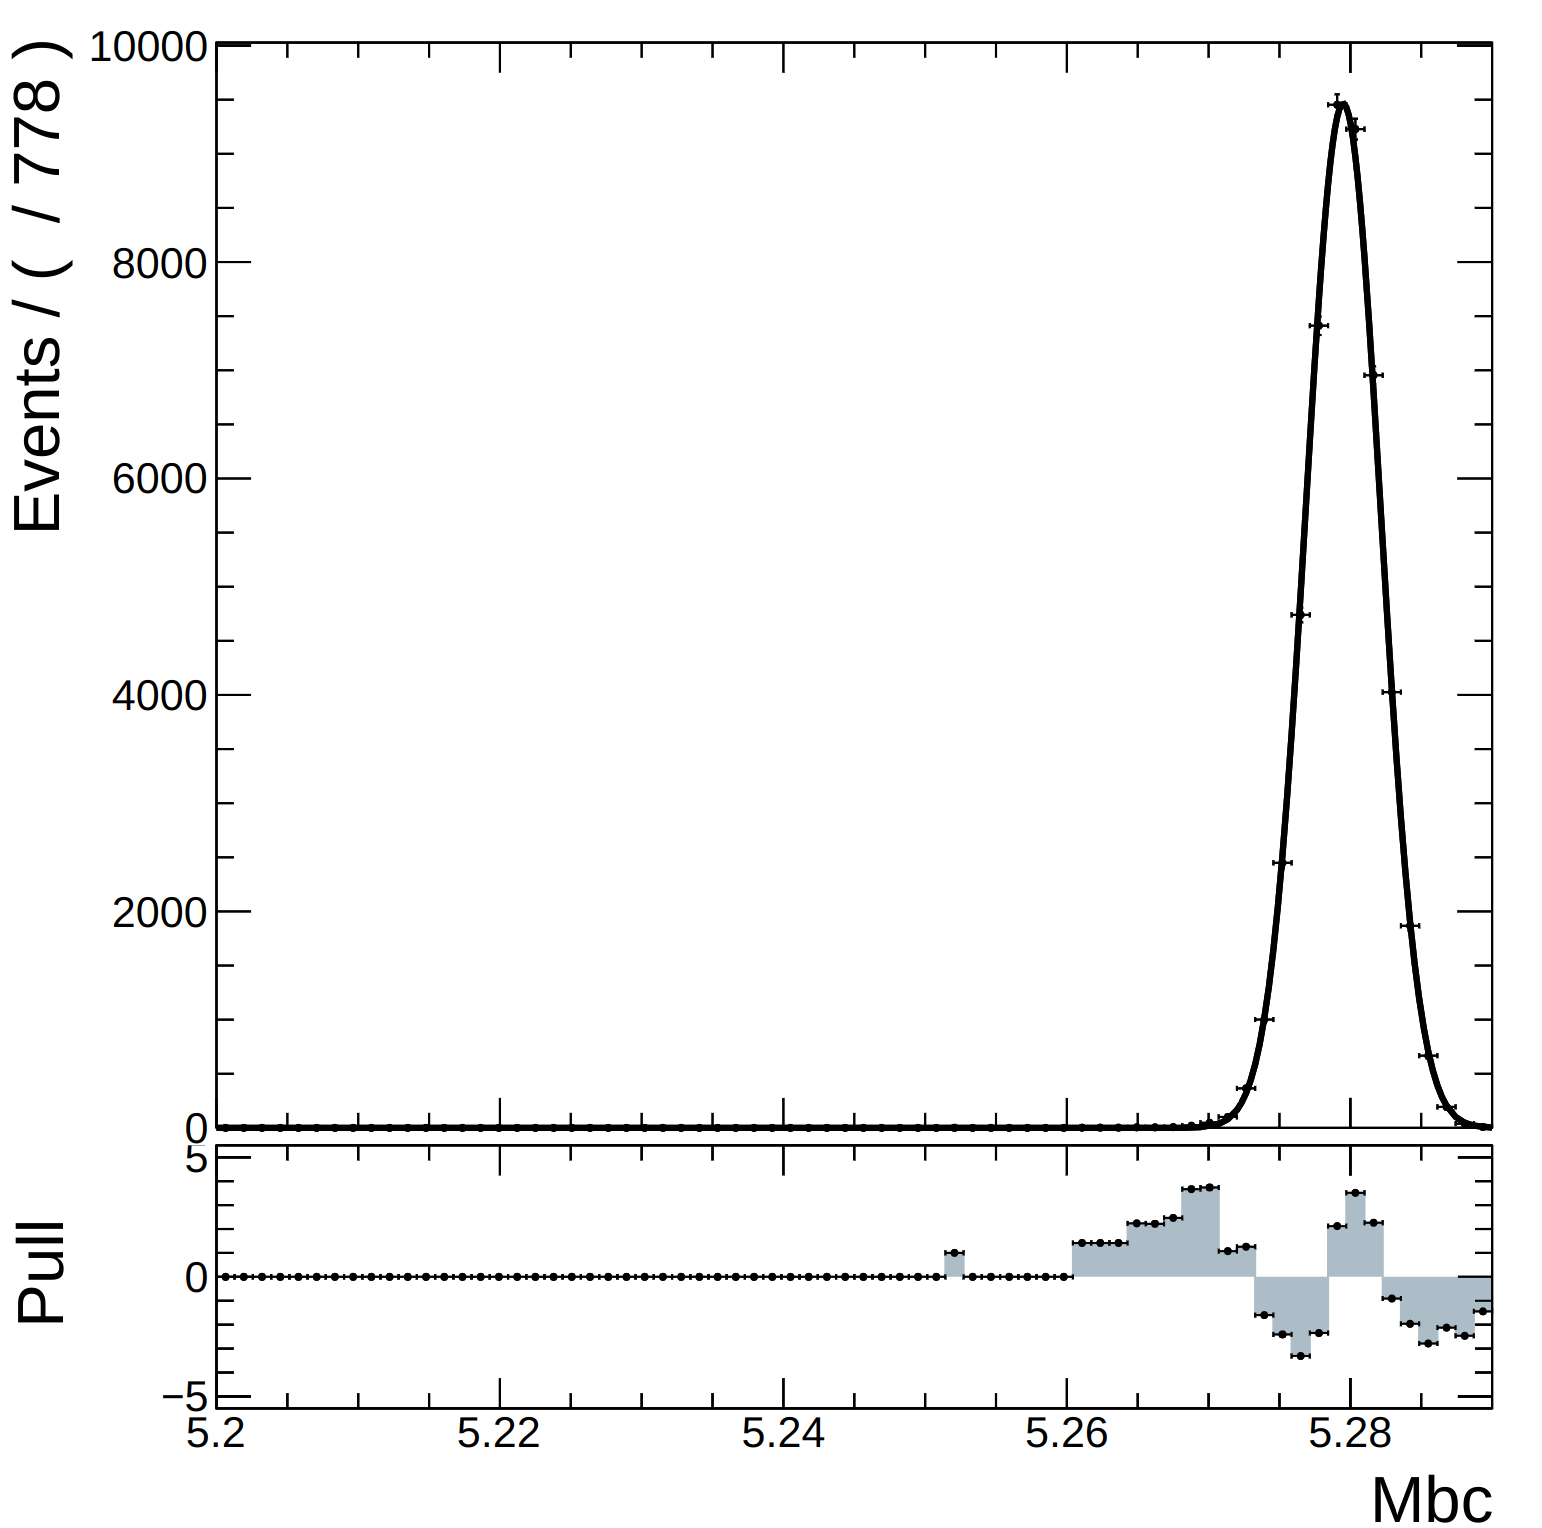
\includegraphics[height=5cm]{mbc-hist}
 		%\label{fig:side:a}
 	\end{minipage}
 	\begin{minipage}[b]{0.5\linewidth}
 		\centering 
 		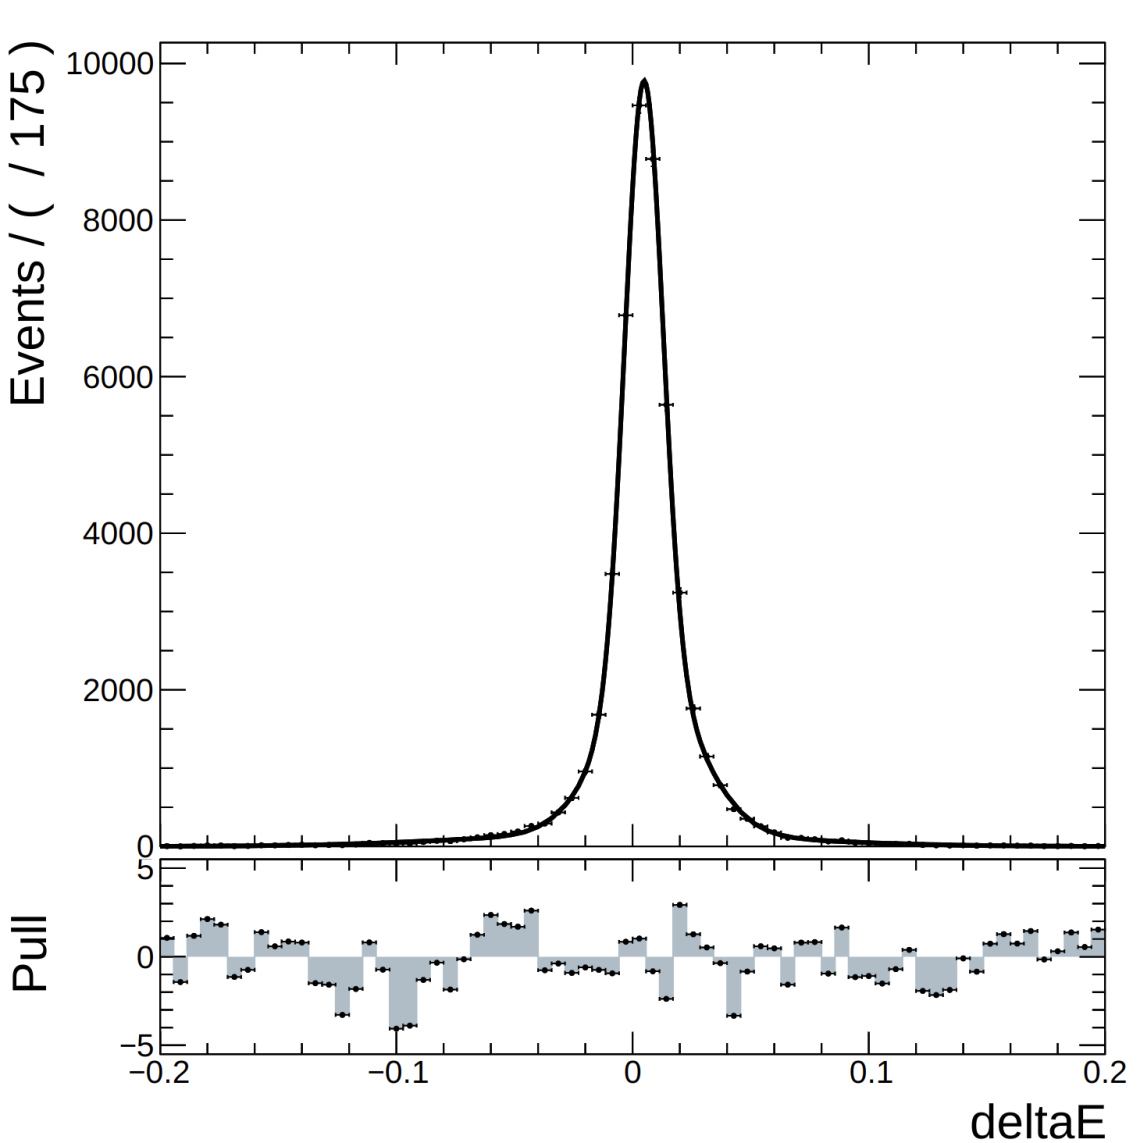
\includegraphics[height=5.2cm]{dE-hist}
 		%\label{fig:side:b}
 	\end{minipage}
 	\caption{The distribution of $M_{bc}$ and $\Delta E$ of signal MC of $B^0 \to K_S^0  K_S^0  K_S^0$ fitted with single and triple Gaussian functions respectively.}
 	\label{fig:mbcde1D}
 \end{figure}
The continuum background is fitted by using off-resonance generic MC to determine the shapes then fix them as constants for 2D fit as shown in Figure \ref{fig:bkgmbcde}.
\begin{figure}[htbp]
	\begin{minipage}[b]{0.5\linewidth}
		\centering 
		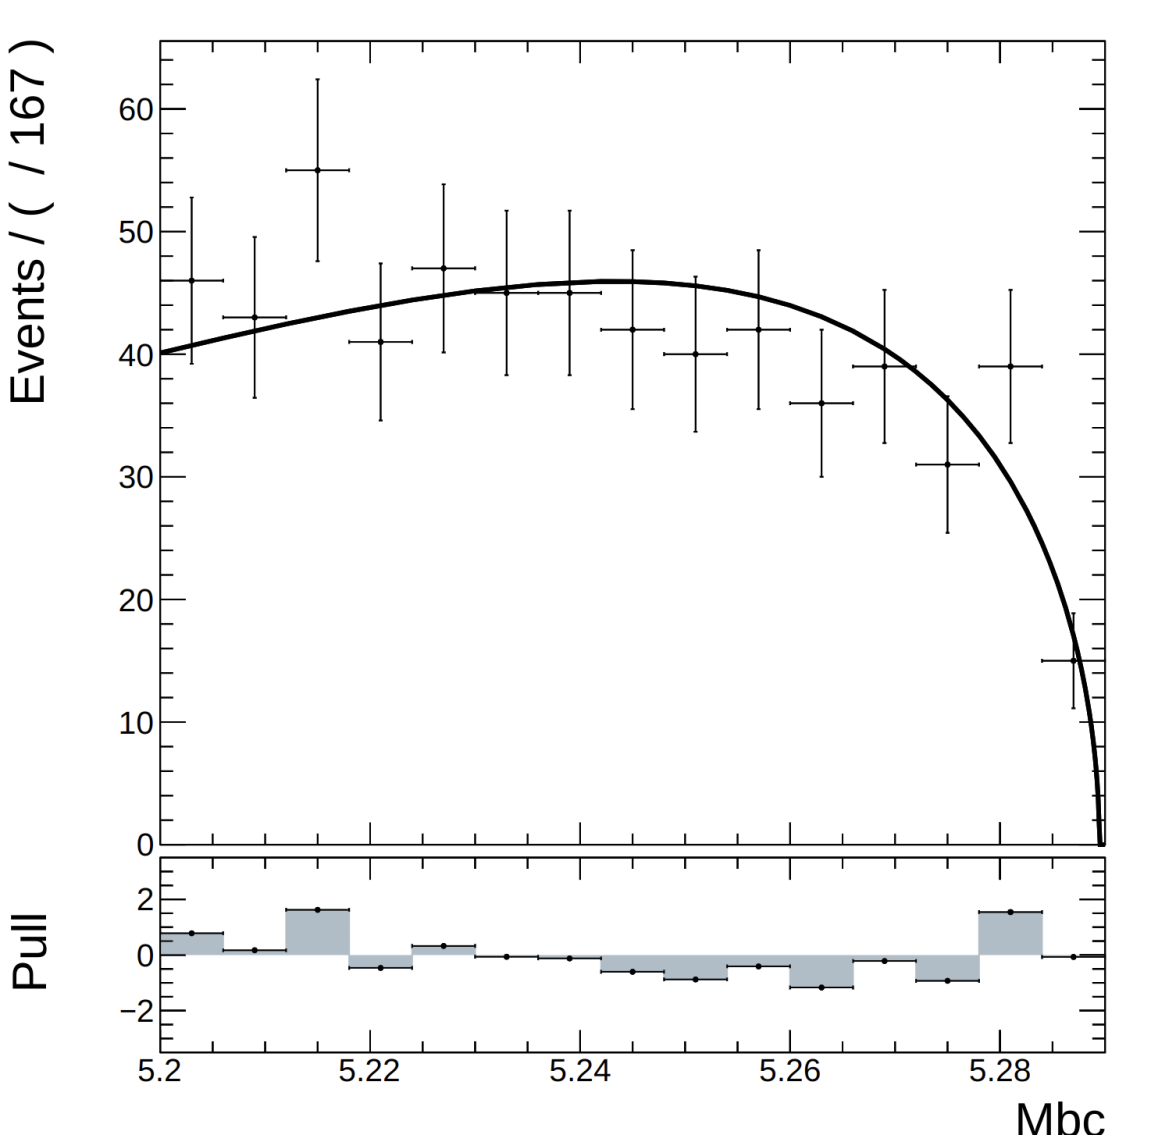
\includegraphics[height=5cm]{figures/mbc-cs-hist}
		\label{}
	\end{minipage}
	\begin{minipage}[b]{0.5\linewidth}
		\centering 
		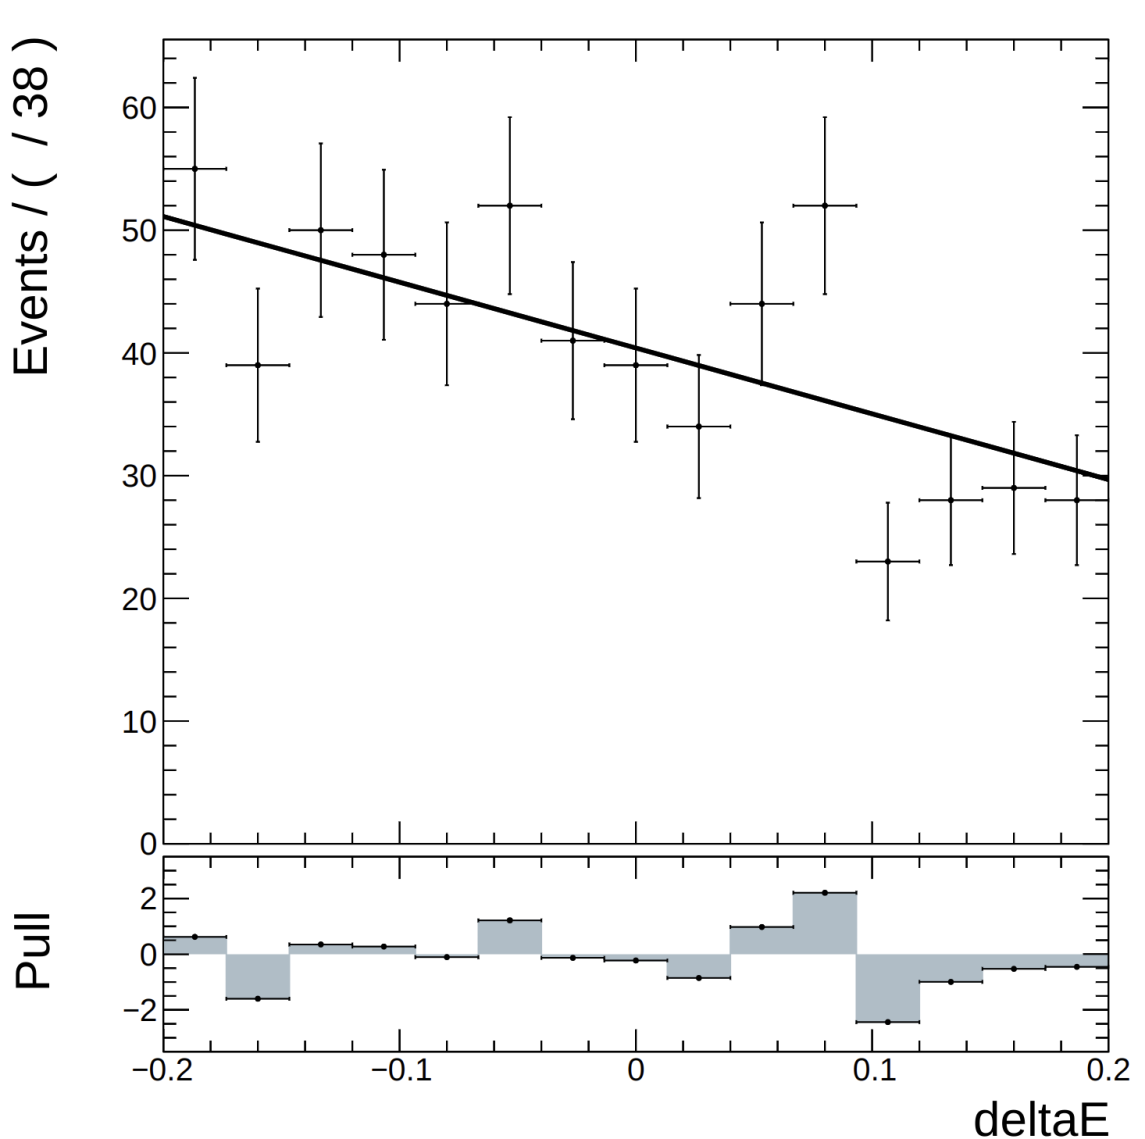
\includegraphics[height=5.2cm]{figures/dE-cs-hist}
		\label{}
	\end{minipage}
	\caption{The distribution of $M_{bc}$ and $\Delta E$ of continuum events in generic MC fitted with Argus and Chebyshev polynomial, respectively.}
	\label{fig:bkgmbcde}
\end{figure}

Then we set the events number for signal and background as floating parameters and use Equation \ref{eq:pmbcde} as 2D fit model on 1 ab$^{-1}$ generic MC and experiment data, which is also done by using unbinned maximum likelihood fit.
For $B^0$ in generic MC, the stacked histogram of each contirbution and the 2D fit result projected on $M_{bc}$ and $\Delta E$ is shown in Figure \ref{fig:2Dgen}.
\begin{figure}[H]
	\begin{minipage}[b]{0.5\linewidth}
		\centering 
		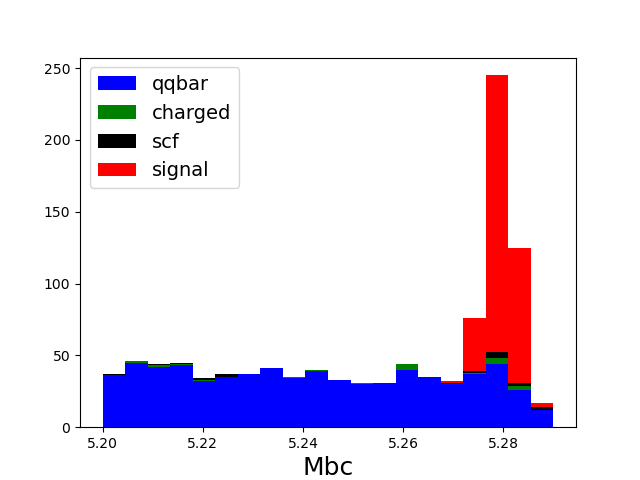
\includegraphics[height=5cm]{figures/hist_stacked_generic_mbc}
		\label{}
	\end{minipage}
	\begin{minipage}[b]{0.5\linewidth}
		\centering 
		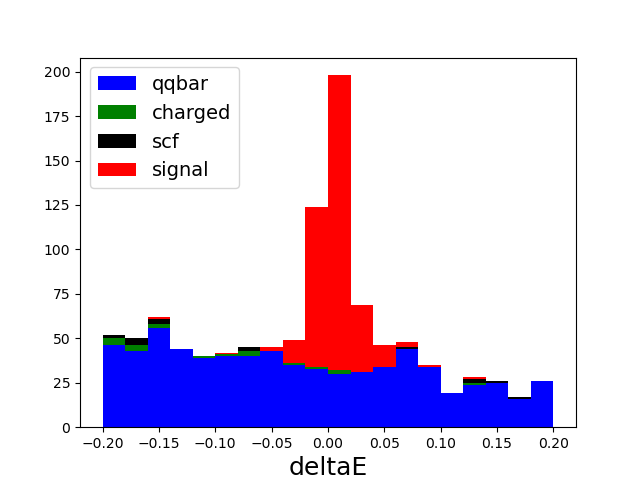
\includegraphics[height=5.2cm]{figures/hist_stacked_generic_dE}
		\label{}
	\end{minipage}
	\begin{minipage}[b]{0.5\linewidth}
		\centering 
		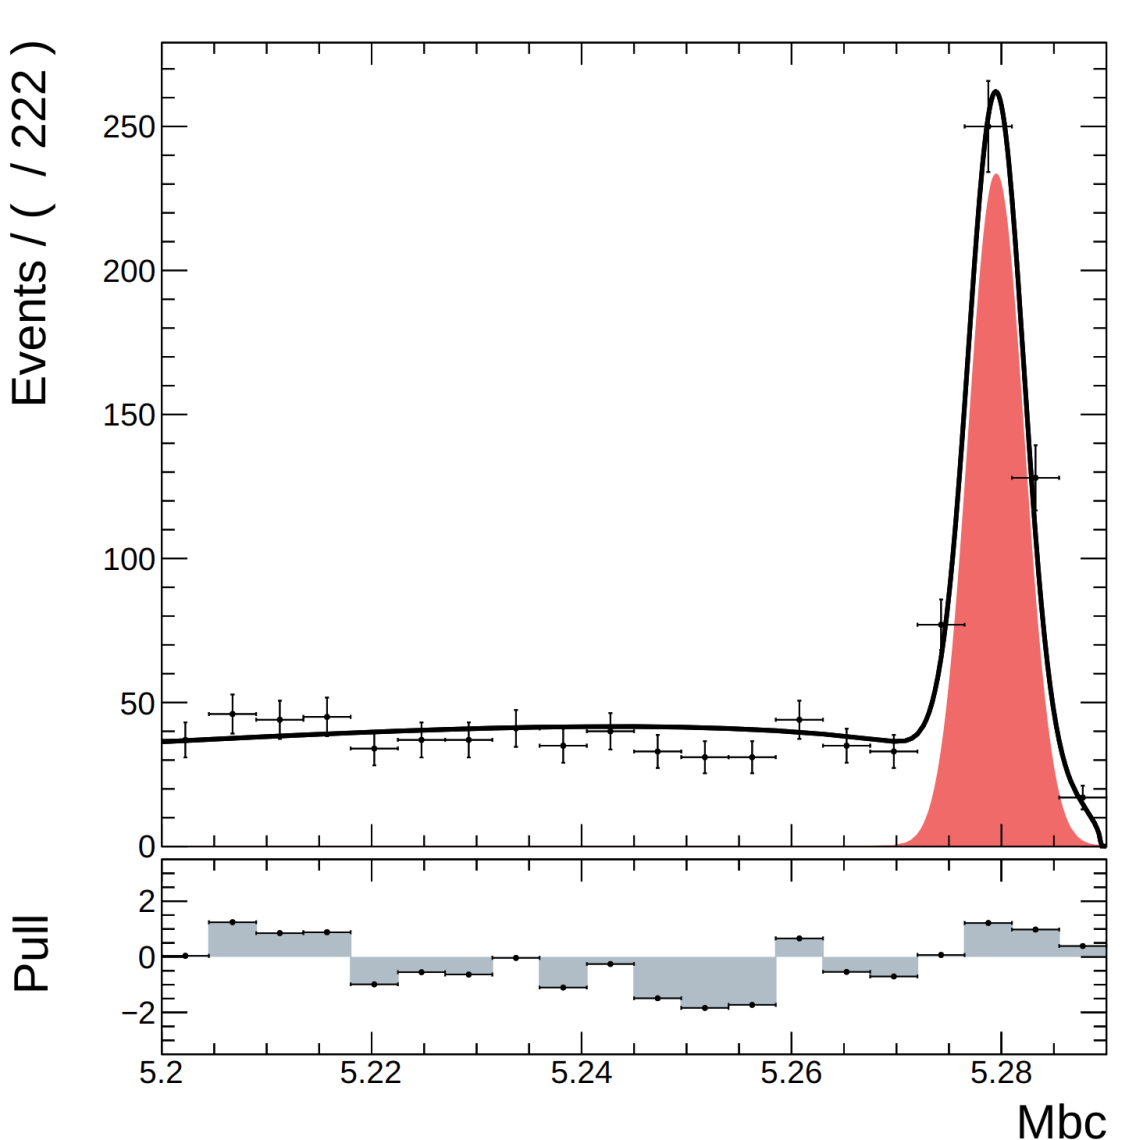
\includegraphics[height=5cm]{figures/mbc-hist-2d}
		\label{}
	\end{minipage}
	\begin{minipage}[b]{0.5\linewidth}
		\centering 
		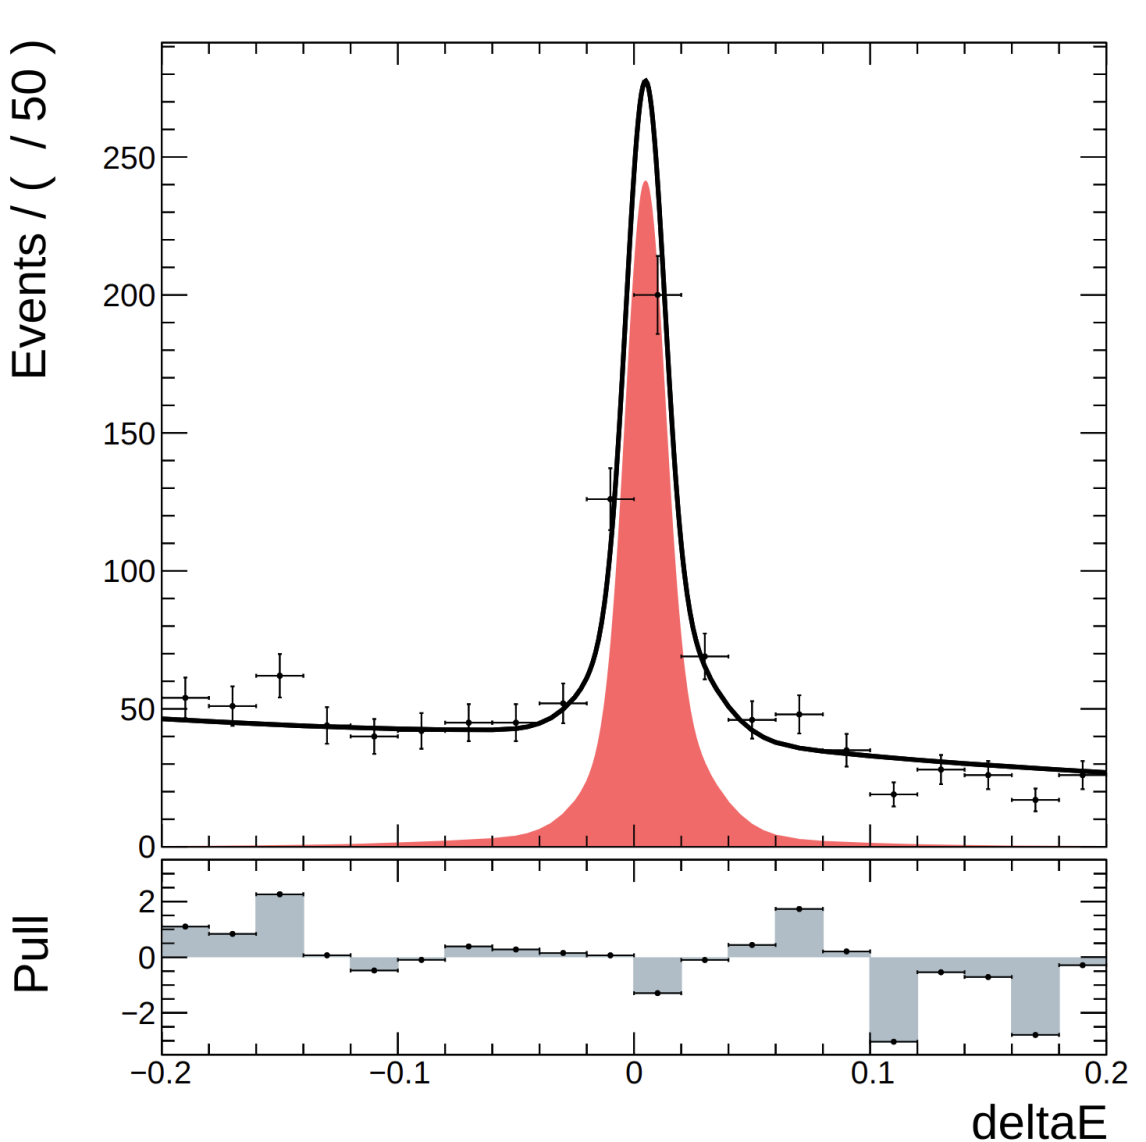
\includegraphics[height=5.2cm]{figures/dE-hist-2d}
		\label{}
	\end{minipage}
	\caption{Top is the stacked plots for generic MC of $M_{bc}$ and $\Delta E$, where each background components are stacked with signal. The bottom is the 2D fit on 1 ab$^{-1}$ generic MC projected on $M_{bc}$ and $\Delta E$, the red is signal component from the fit result in both plots.}
	\label{fig:2Dgen}
\end{figure}

Before perform fitting on experiment data, the distribution of $K_S^0$ invariant mass from the reconstructed $B^0$ candidates is compared between generic MC and experiment data. The distributions are shown in Figure \ref{fig:b0ksmass}, where the generic MC is scaled to the luminosity of experiment data and an agreement within $\sim 1\sigma$ is observed on average.

The 2D fit of experiment data projected on $M_{bc}$ and $\Delta E$ is in Figure \ref{fig:2Ddata}.  
\begin{figure}[htbp]
\begin{minipage}[b]{0.5\linewidth}
	\centering 
	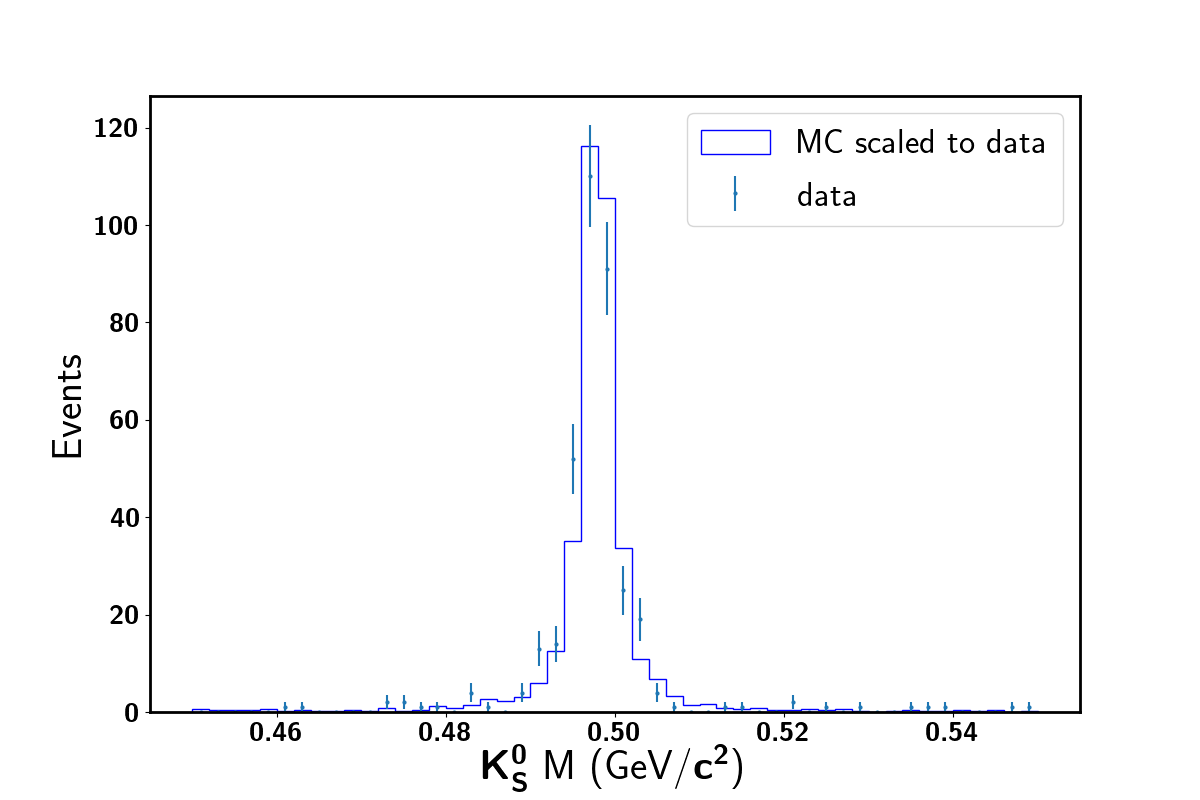
\includegraphics[height=6cm]{figures/best_KsM}	
\end{minipage}
\begin{minipage}[b]{0.5\linewidth}
	\centering 
	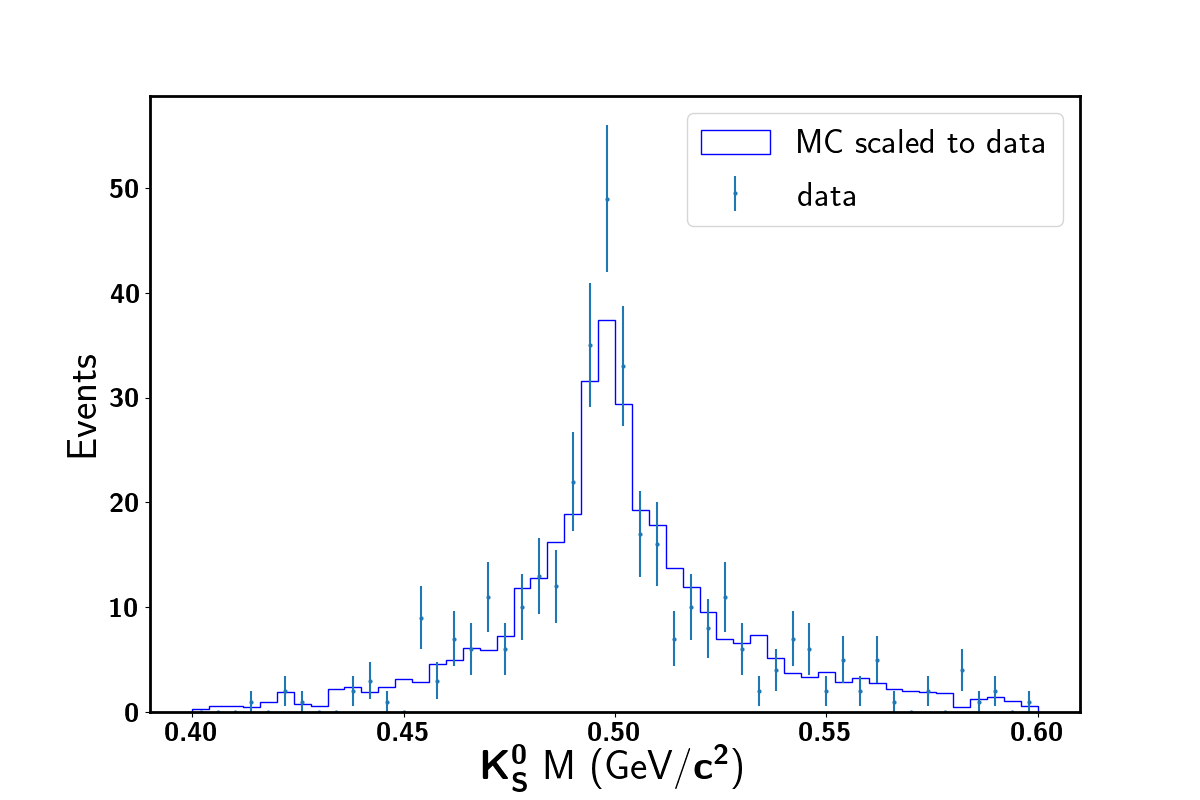
\includegraphics[height=6cm]{figures/best_KsInvM}	
\end{minipage}
\caption{Invariant mass before(left) and after vertext fit(right) from generic MC and experiment data.}
\label{fig:b0ksmass}
\end{figure}

\begin{figure}[htbp]
	\begin{minipage}[b]{0.5\linewidth}
		\centering 
		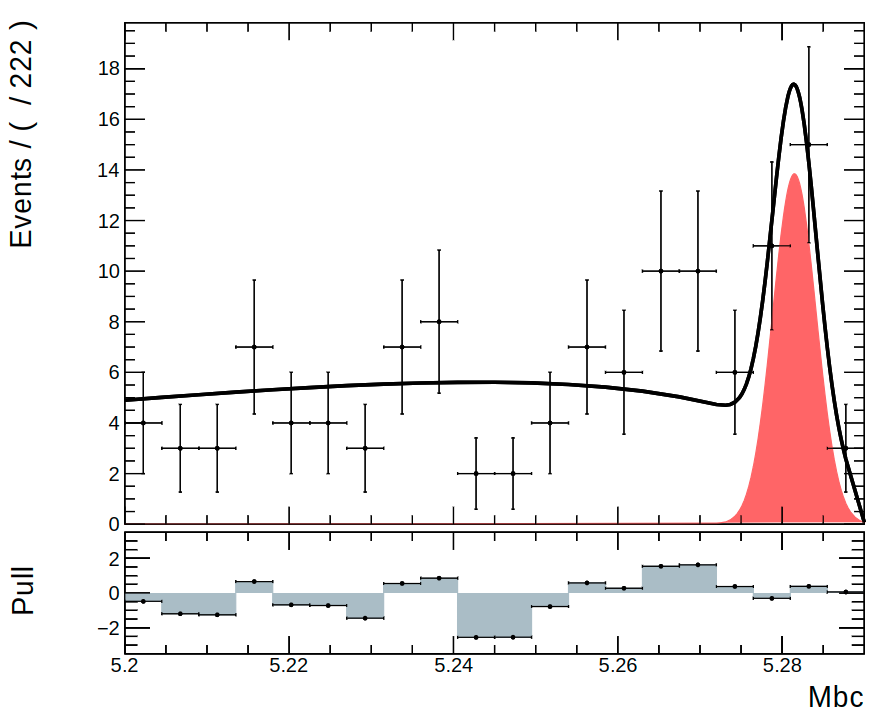
\includegraphics[height=5cm]{figures/mbc_data_new}
		\label{}
	\end{minipage}
	\begin{minipage}[b]{0.5\linewidth}
		\centering 
		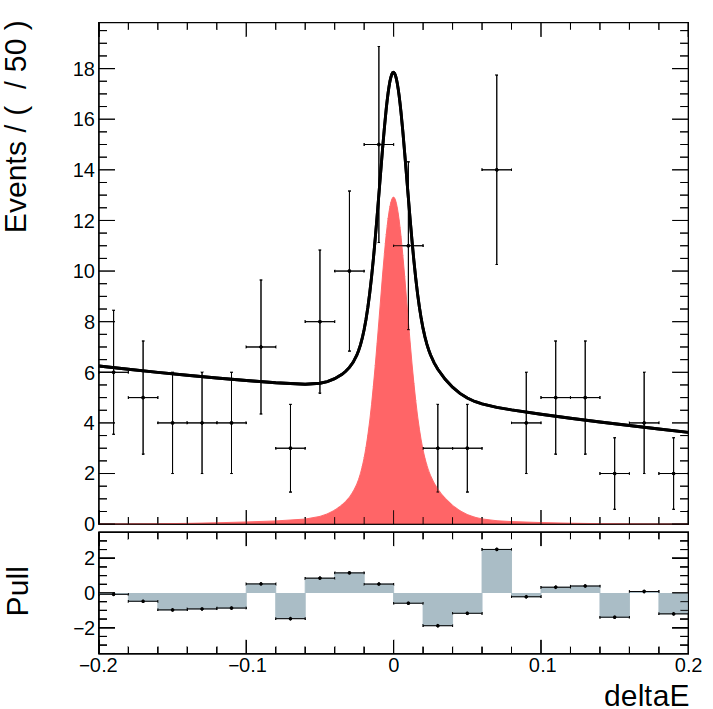
\includegraphics[height=5.2cm]{figures/dE_data_new}
		\label{}
	\end{minipage}
\caption{$M_{bc}$ and $\Delta E$ 2D fit on 62.8 fb$^{-1}$data, the red is the signal component.}
\label{fig:2Ddata}
\end{figure}

 The number of signal events is extracted by the integral of fit model over the signal region which is defined as $5.27 < M_{bc} < 5.29 $ GeV and $-0.1 < \Delta E < 0.1$ GeV.
 The expected signal events with $\sim 35\%$ efficiency is calculated as Equation \ref{eq:b0nsig}.
 \begin{equation}\label{eq:b0nsig}
 \mathcal{B}(B^0 \to K_S^0  K_S^0  K_S^0)=
 \frac{N_{sig}}{\mathcal{B}(K_S^0\to \pi^+\pi^-)^3\times
 	\epsilon_{rec}\times N_{B\bar{B}}}
 \end{equation}
 In 1 ab$^{-1}$ generic MC, the expected signal number is $7.7\times 10^8 \times 6\times 10^{-6} \times 21\% \times 35\% \simeq 339$. The 2D fit result from $M_{bc}$ and $\Delta E$ yields $341\pm 20$ events which agrees with expected number within $1\sigma$. The event number in sideband defined as $M_{bc}<5.26$ GeV in generic MC is 507. Compared to Belle result with $772\times 10^6$ ($\sim$ 1 ab$^{-1}$) $B\overline{B}$ pairs used, signal from data yields $327\pm 19$. In 62.8 fb$^{-1}$ data fit in Belle II, we extract $N_{sig} = 17.4 \pm 4.2$ in signal region. The sideband region $M_{bc}<5.26$ GeV contains 60 events in data. 
 
To check linearity of the event number fitted from the $M_{bc}$ and $\Delta E$ in this low statistics case, we extract the fraction of continuum backgrounds from generic MC sample rescaled to the experimental data luminosity, which includes about 46 continuum events. Then the number of signal events from 5 to 30 with 5 events per step are injected into the continuum events, to perform the $M_{bc}$ and $\Delta E$ fit to check the output signal events number. The $M_{bc}$ and $\Delta E$ distributions and fit in each injection test are shown in Figure \ref{fig:2Dinject}. The fitted signal and background events depending on the injected numbers (linearity test ) are presented in Figure \ref{fig:2Dinjectline}, where the dependence on both signal and background events number are fitted with linear functions. The fit results show a good linearity on the input and output of signal numbers while the background numbers remain constant close to the input number.

\begin{figure}[htpb]
	
	\begin{subfigure}{0.5\linewidth}
		\includegraphics[page=1,height=5cm]{figures/injection_sig_5/ds_gen_Mbc_2D.pdf}
		\caption{signal injected: 5}
	\end{subfigure}
	\begin{subfigure}{0.5\linewidth}
		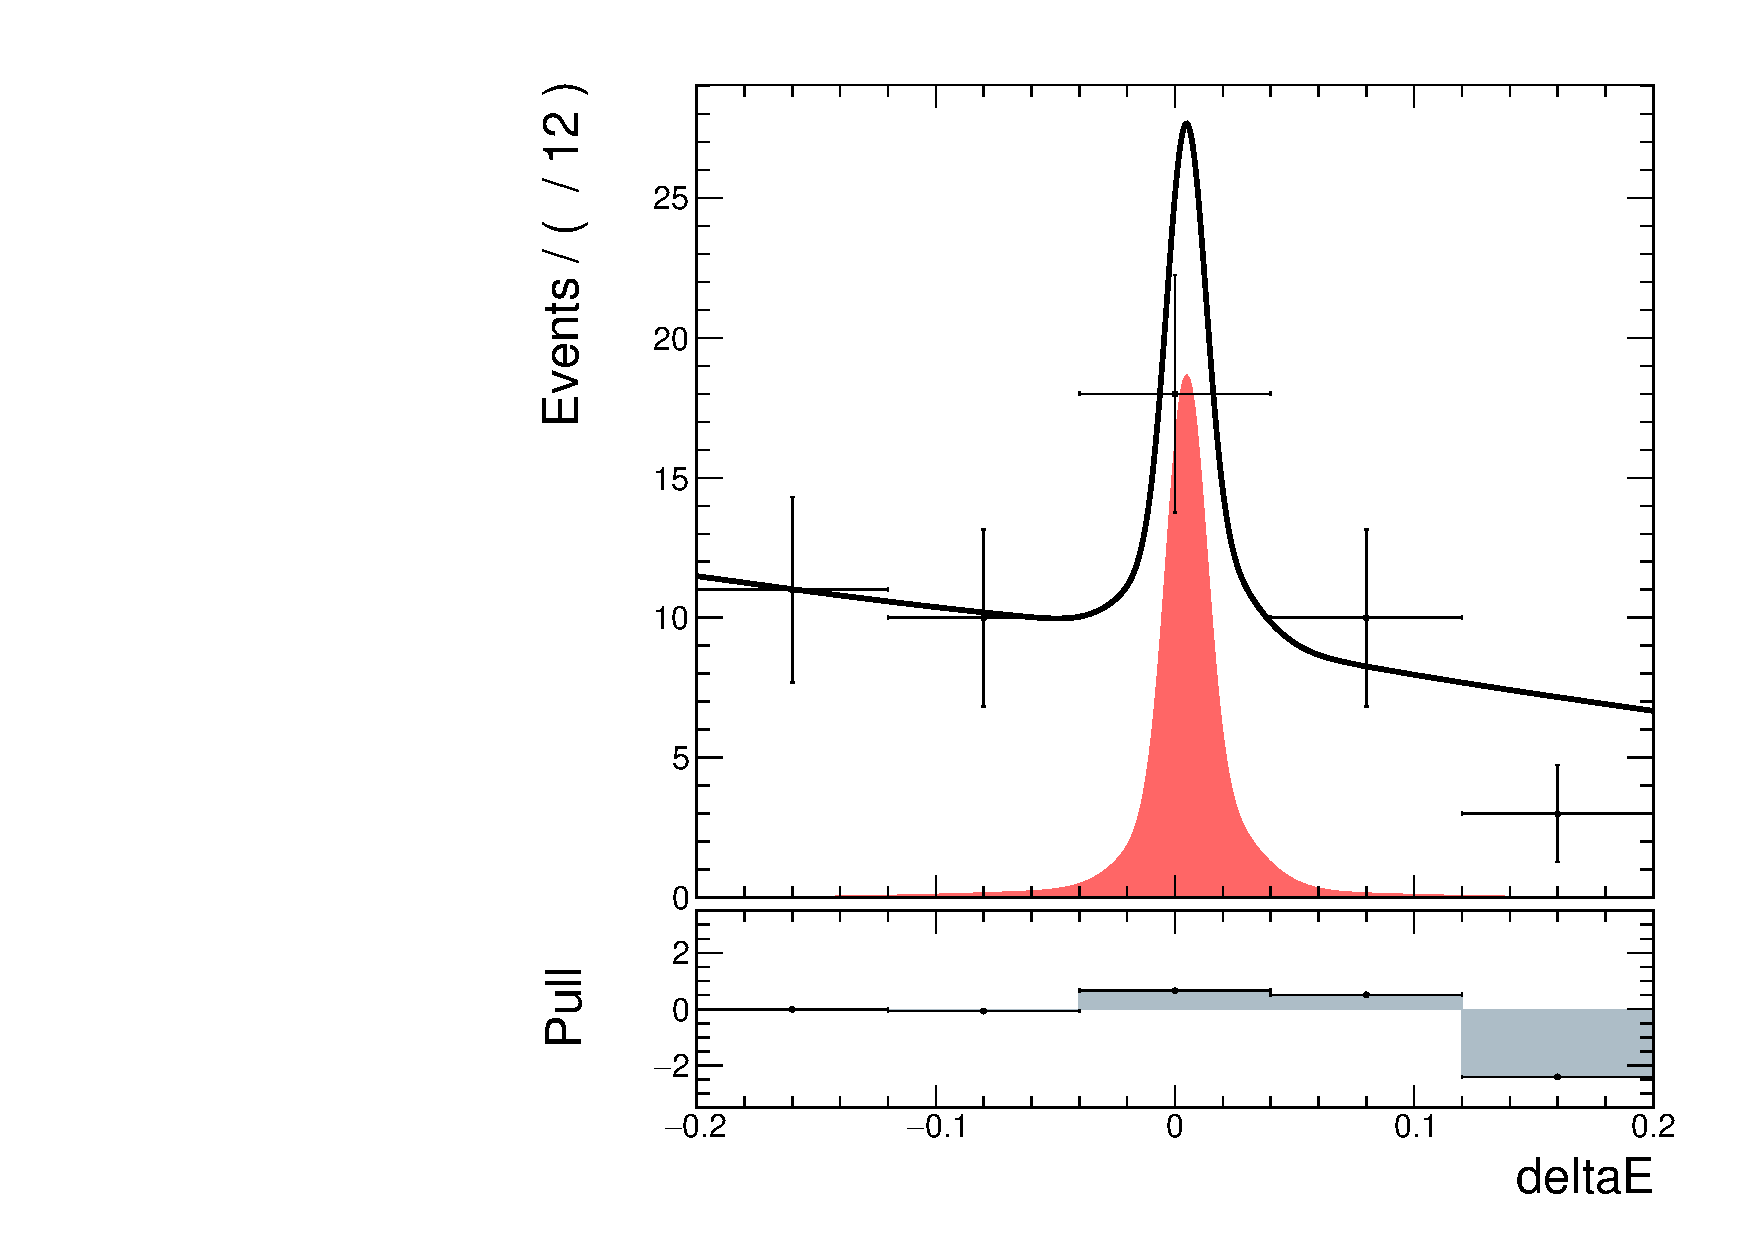
\includegraphics[page=1,height=5cm]{figures/injection_sig_5/ds_gen_deltaE_2D.pdf}
		\caption{signal injected: 5}
	\end{subfigure}
	\begin{subfigure}{0.5\linewidth}
		\includegraphics[page=1,height=5cm]{figures/injection_sig_10/ds_gen_Mbc_2D.pdf}
		\caption{signal injected: 10}
	\end{subfigure}
	\begin{subfigure}{0.5\linewidth}
		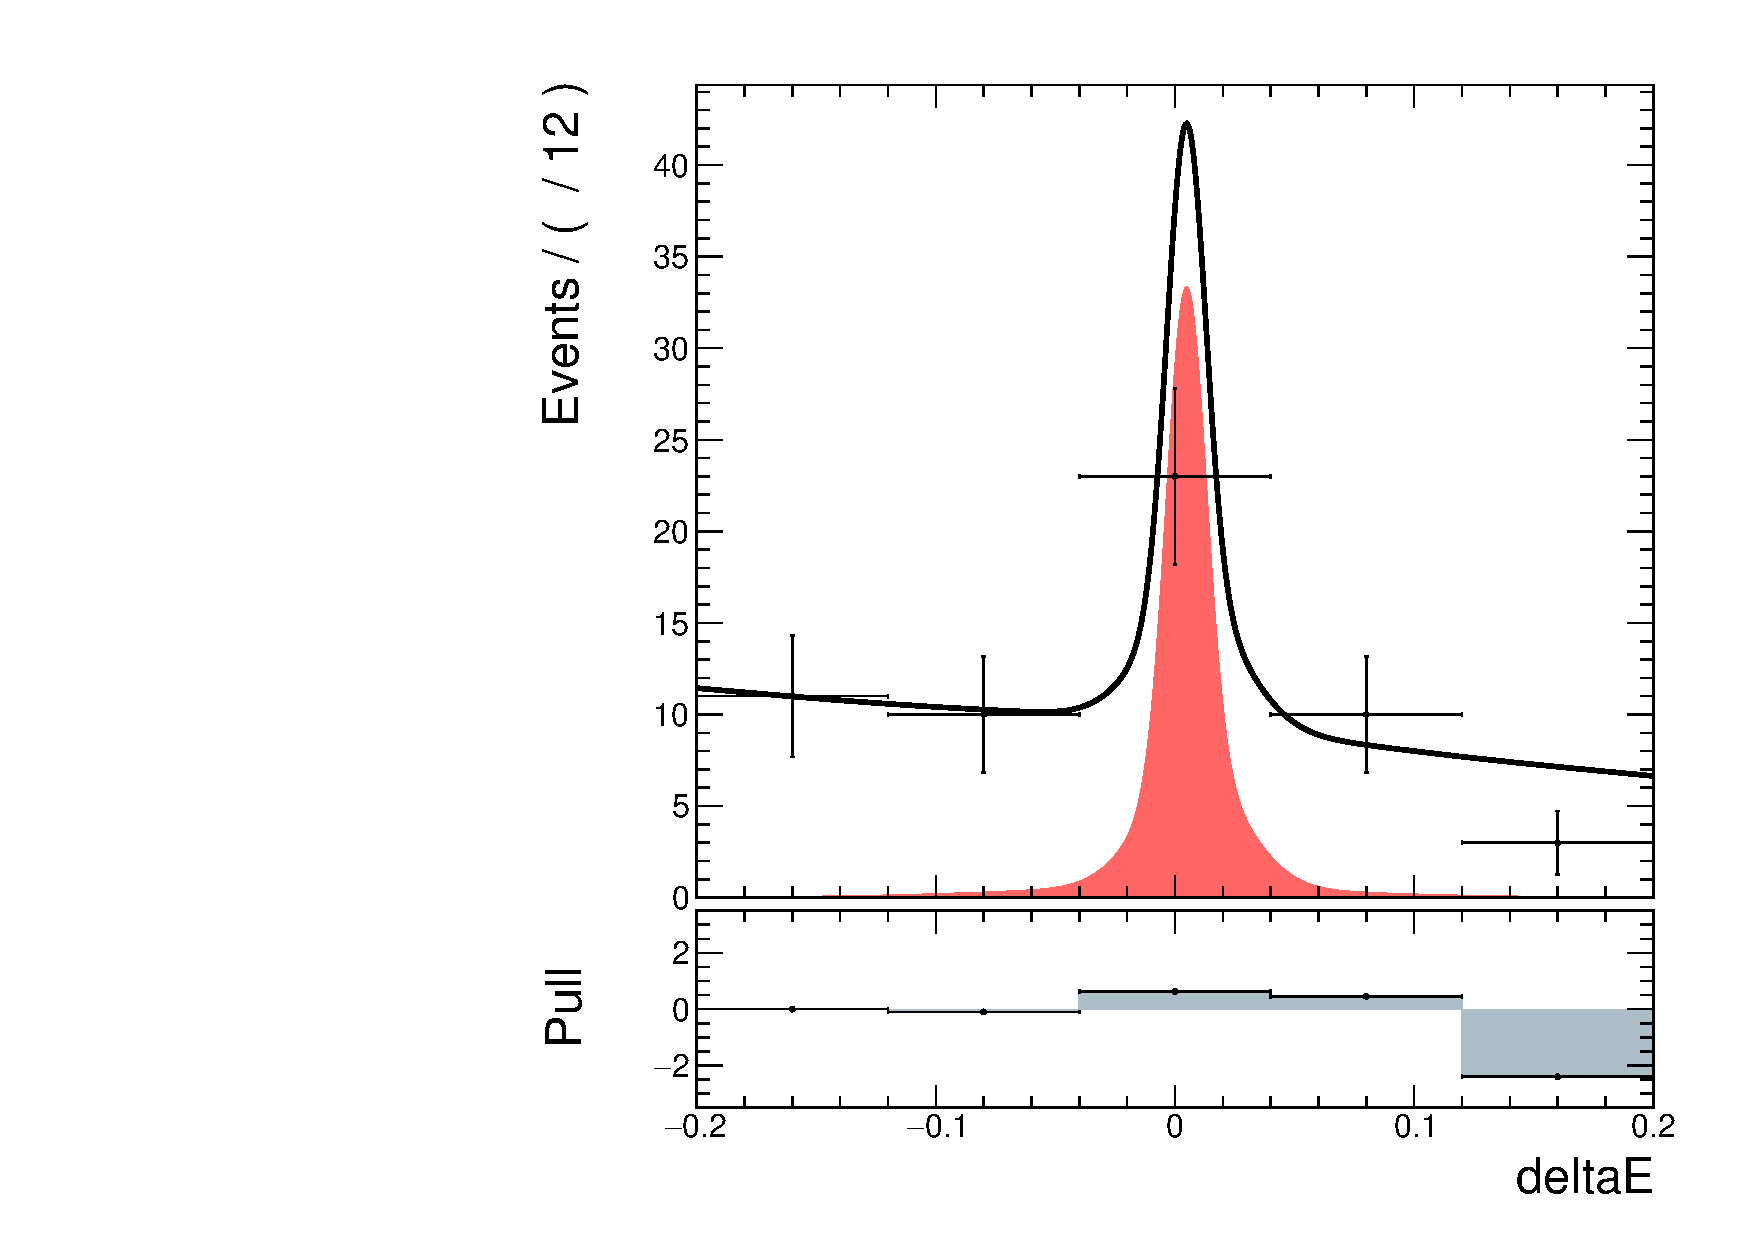
\includegraphics[page=1,height=5cm]{figures/injection_sig_10/ds_gen_deltaE_2D.pdf}
		\caption{signal injected: 10}
	\end{subfigure}
	\begin{subfigure}{0.5\linewidth}
		\includegraphics[page=1,height=5cm]{figures/injection_sig_15/ds_gen_Mbc_2D.pdf}
		\caption{signal injected: 15}
	\end{subfigure}
	\begin{subfigure}{0.5\linewidth}
		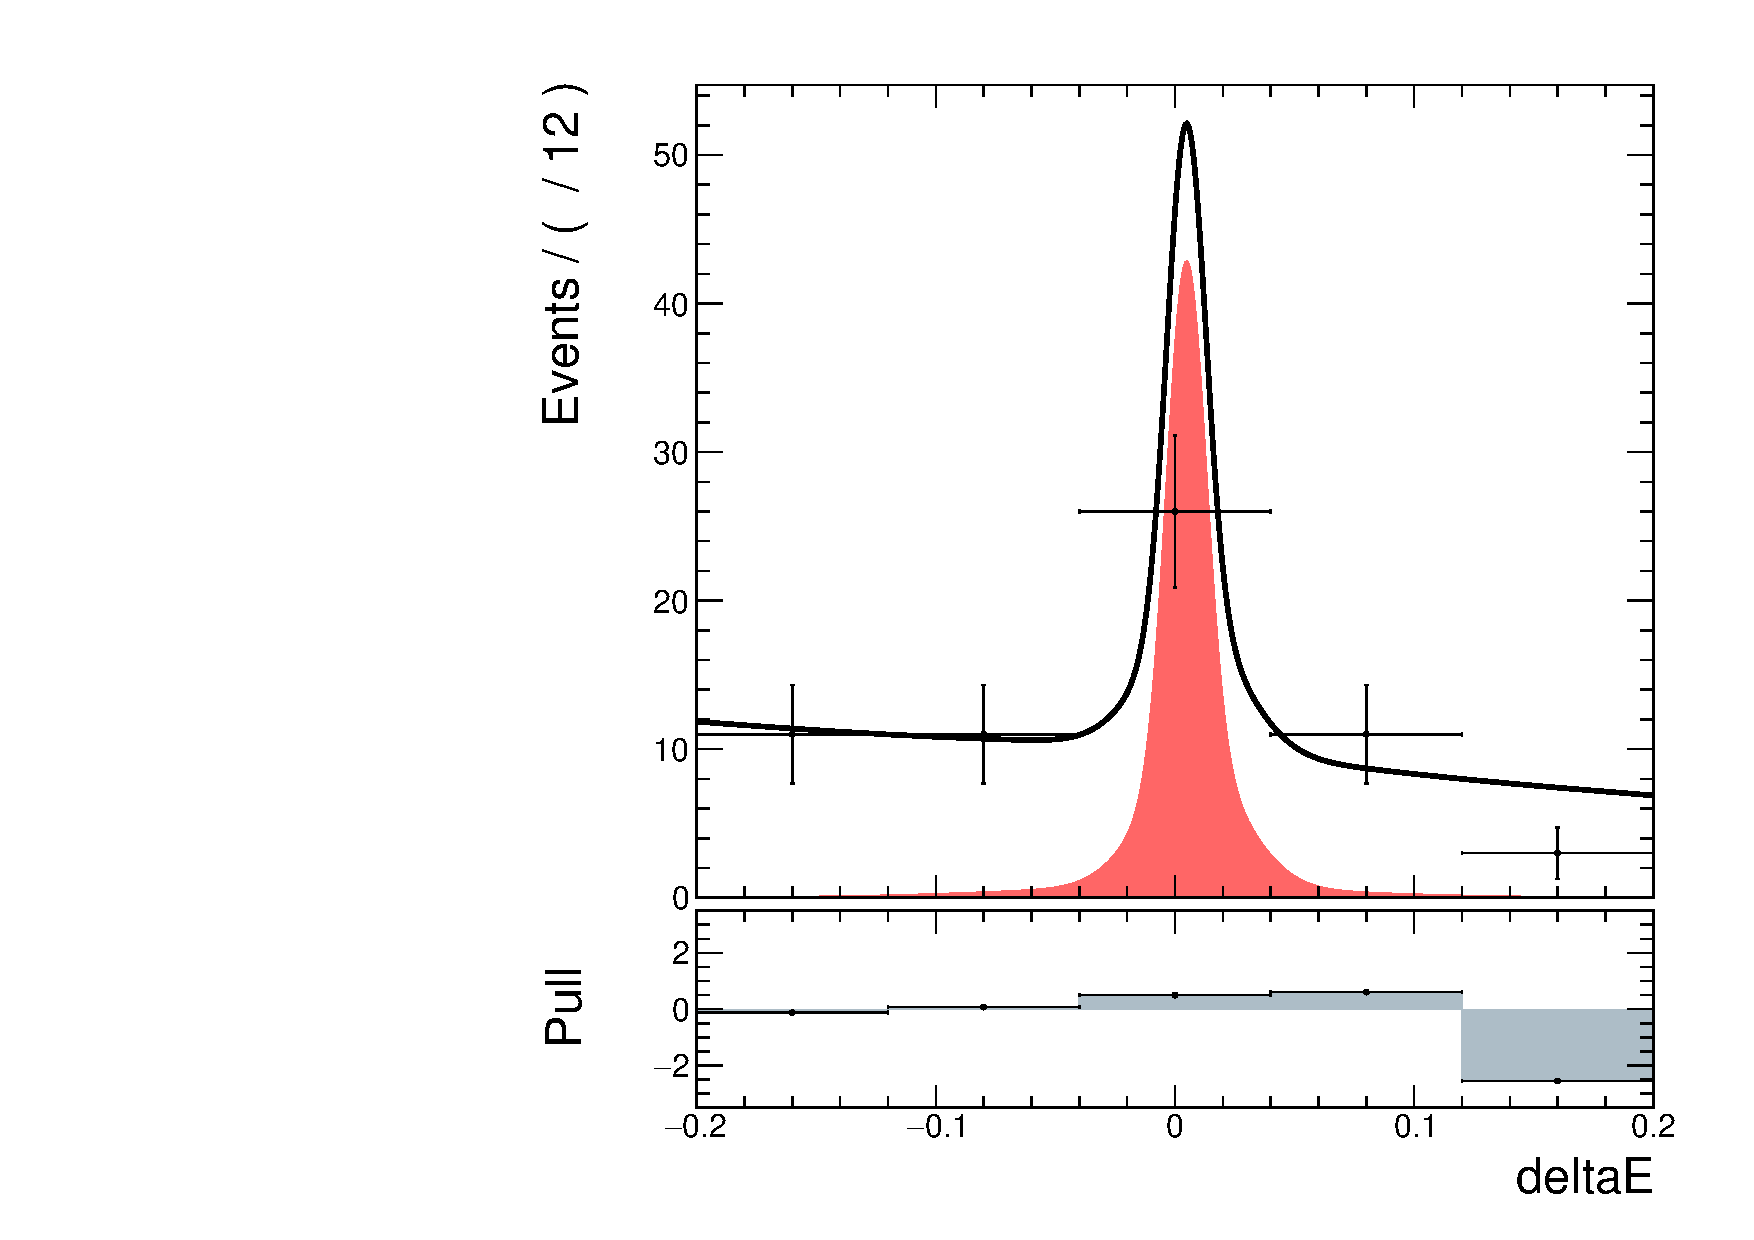
\includegraphics[page=1,height=5cm]{figures/injection_sig_15/ds_gen_deltaE_2D.pdf}
		\caption{signal injected: 15}
	\end{subfigure}
\end{figure}

\begin{figure}[htpb]
	\ContinuedFloat
	\begin{subfigure}{0.5\linewidth}
		\includegraphics[page=1,height=5cm]{figures/injection_sig_20/ds_gen_Mbc_2D.pdf}
		\caption{signal injected: 20}
	\end{subfigure}
	\begin{subfigure}{0.5\linewidth}
		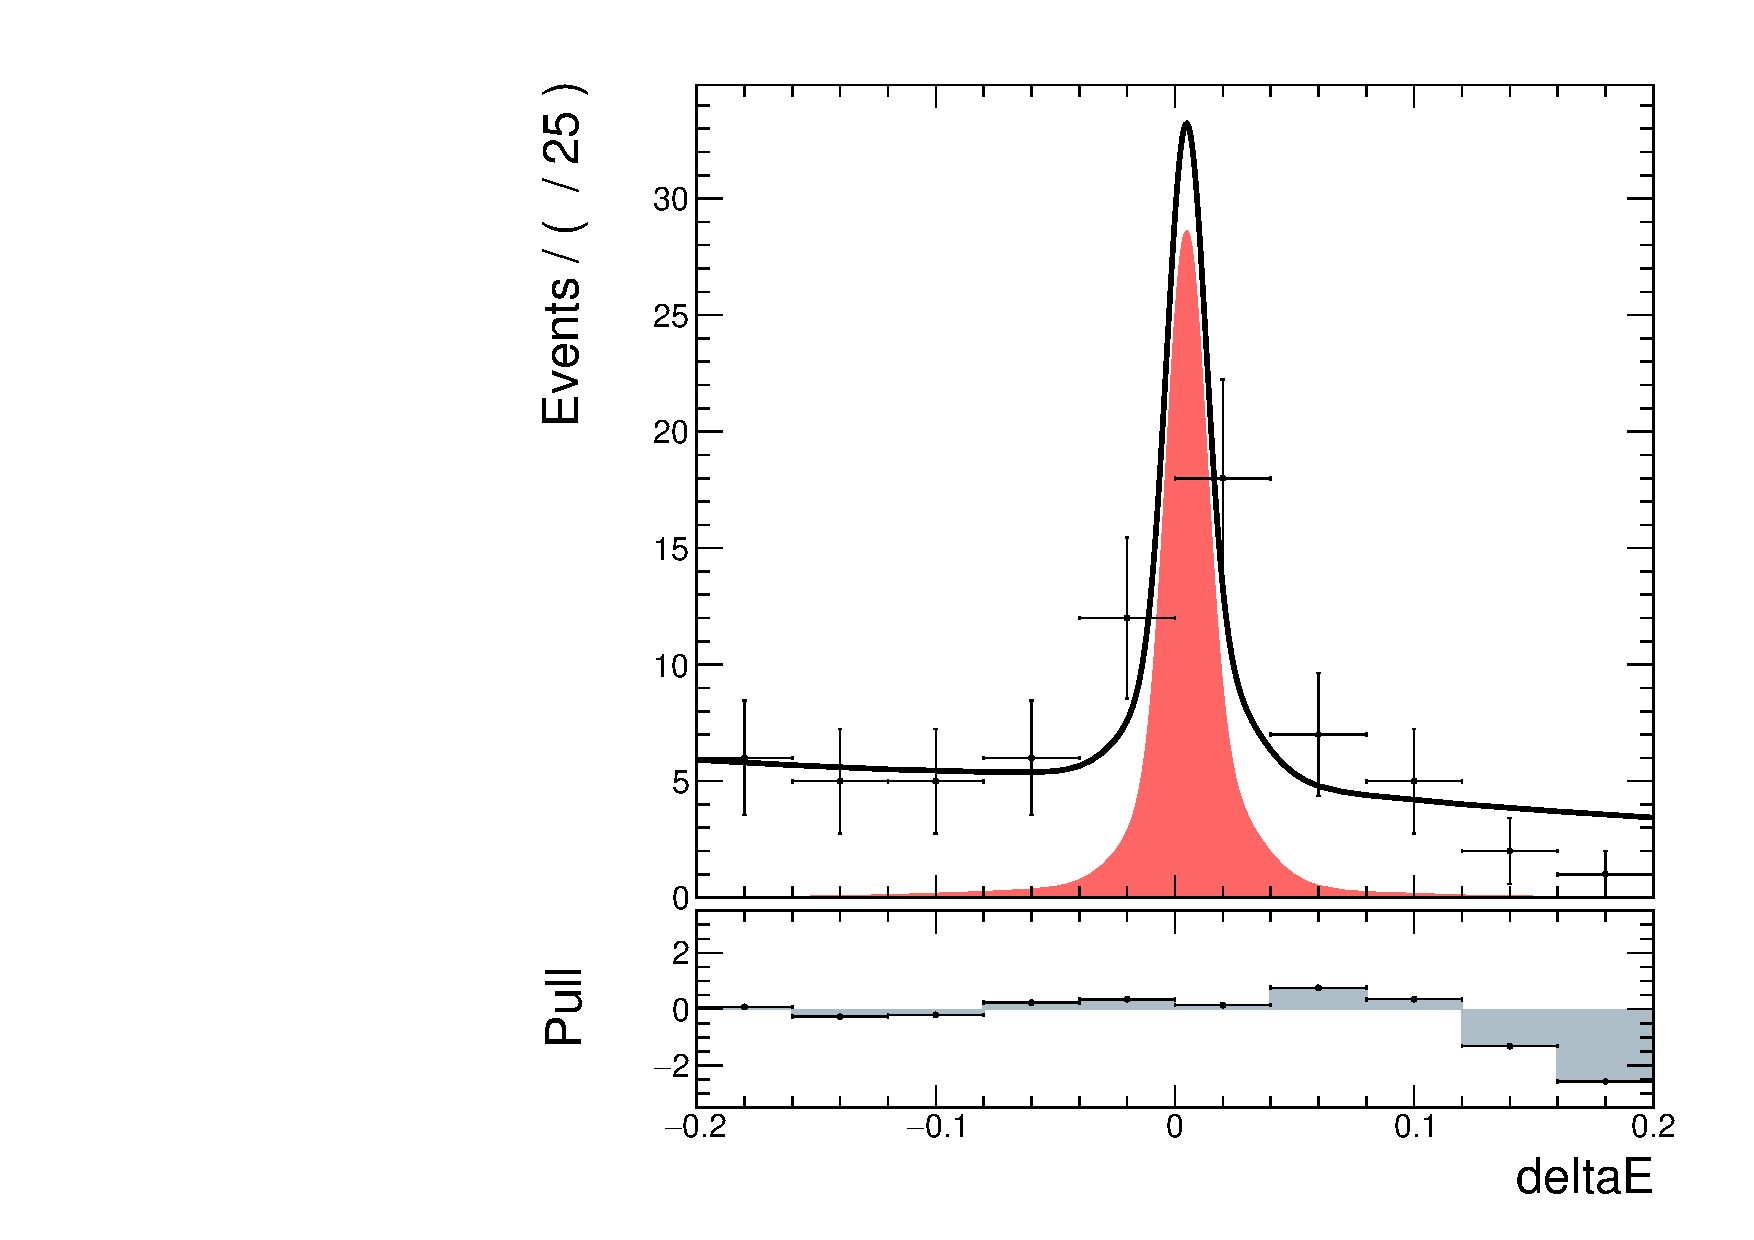
\includegraphics[page=1,height=5cm]{figures/injection_sig_20/ds_gen_deltaE_2D.pdf}
		\caption{signal injected: 20}
	\end{subfigure}
	
	\begin{subfigure}{0.5\linewidth}
		\includegraphics[page=1,height=5cm]{figures/injection_sig_25/ds_gen_Mbc_2D.pdf}
		\caption{signal injected: 25}
	\end{subfigure}
	\begin{subfigure}{0.5\linewidth}
		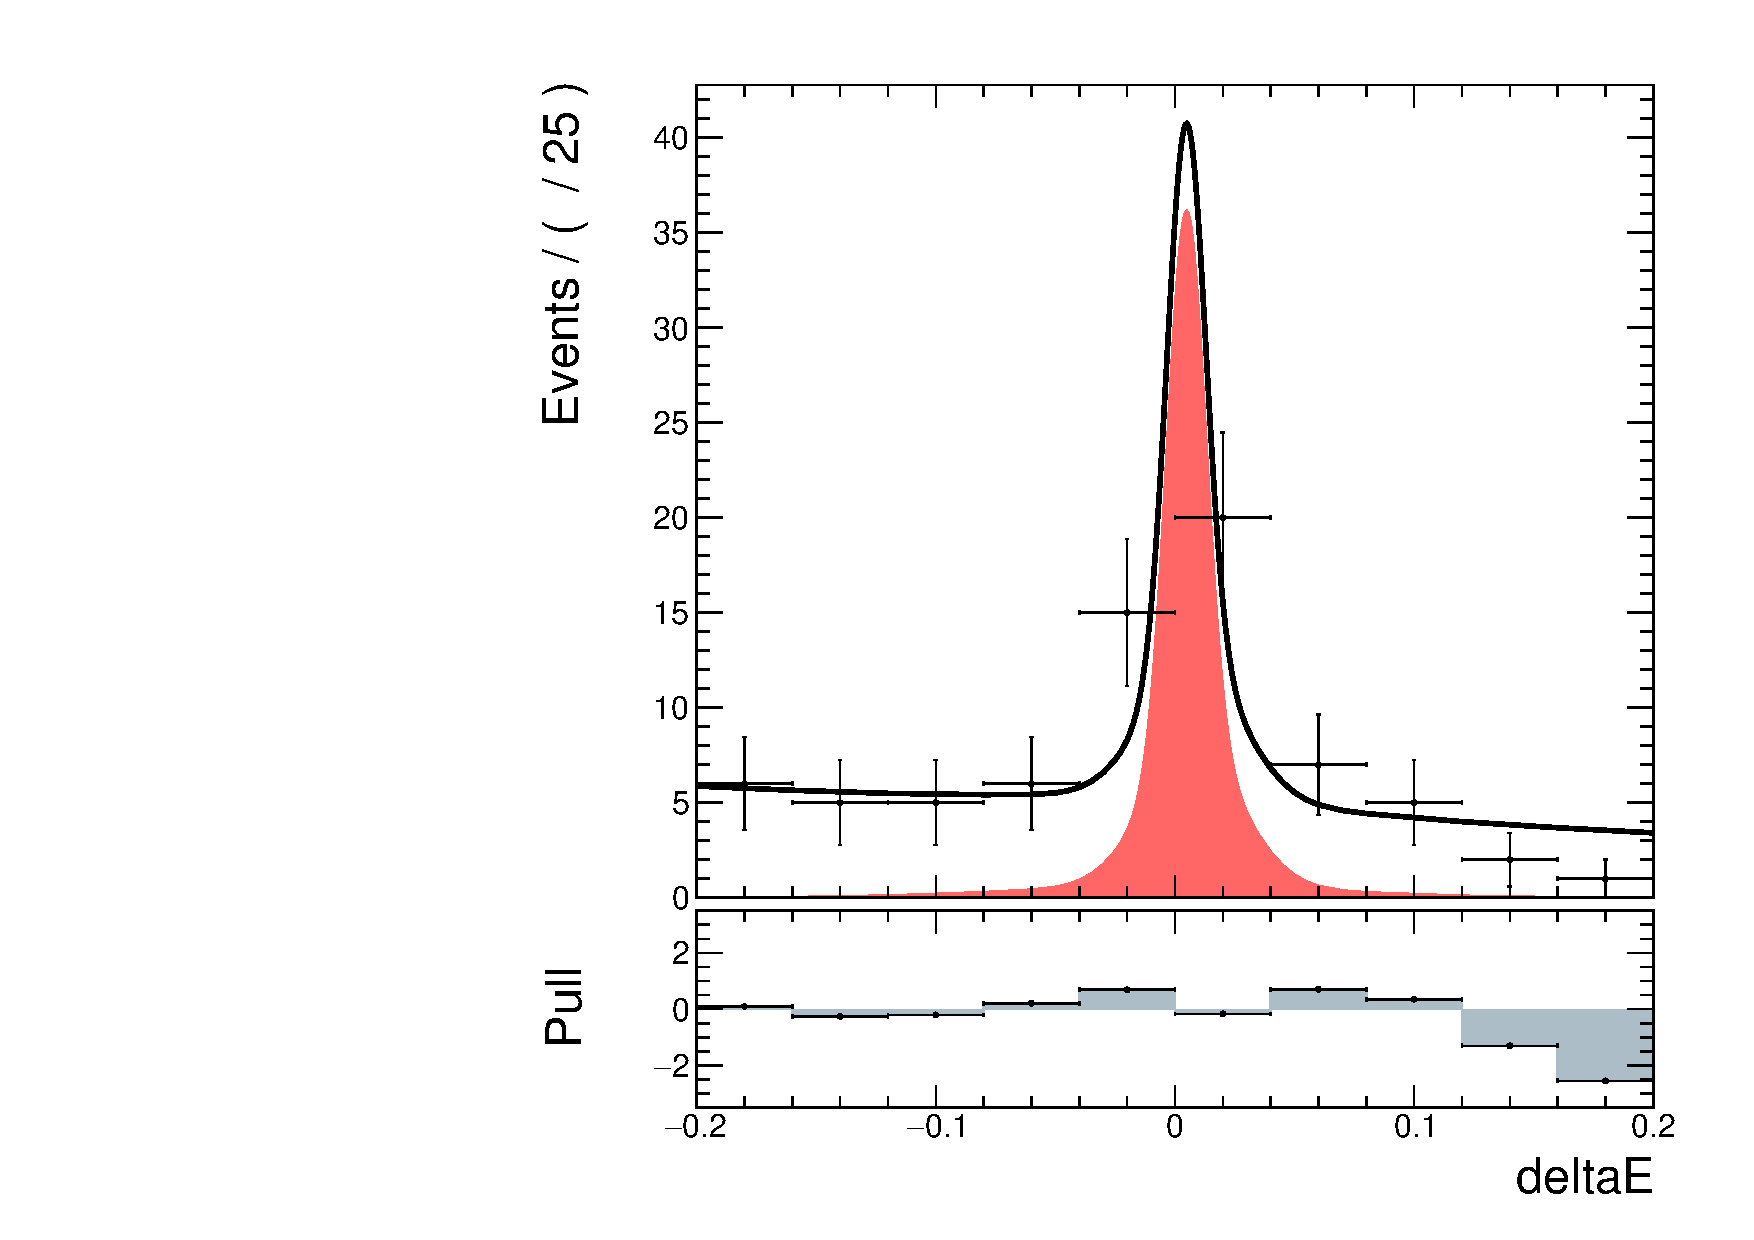
\includegraphics[page=1,height=5cm]{figures/injection_sig_25/ds_gen_deltaE_2D.pdf}
		\caption{signal injected: 25}
	\end{subfigure}
	\begin{subfigure}{0.5\linewidth}
		\includegraphics[page=1,height=5cm]{figures/injection_sig_30/ds_gen_Mbc_2D.pdf}
		\caption{signal injected: 30}
	\end{subfigure}
	\begin{subfigure}{0.5\linewidth}
		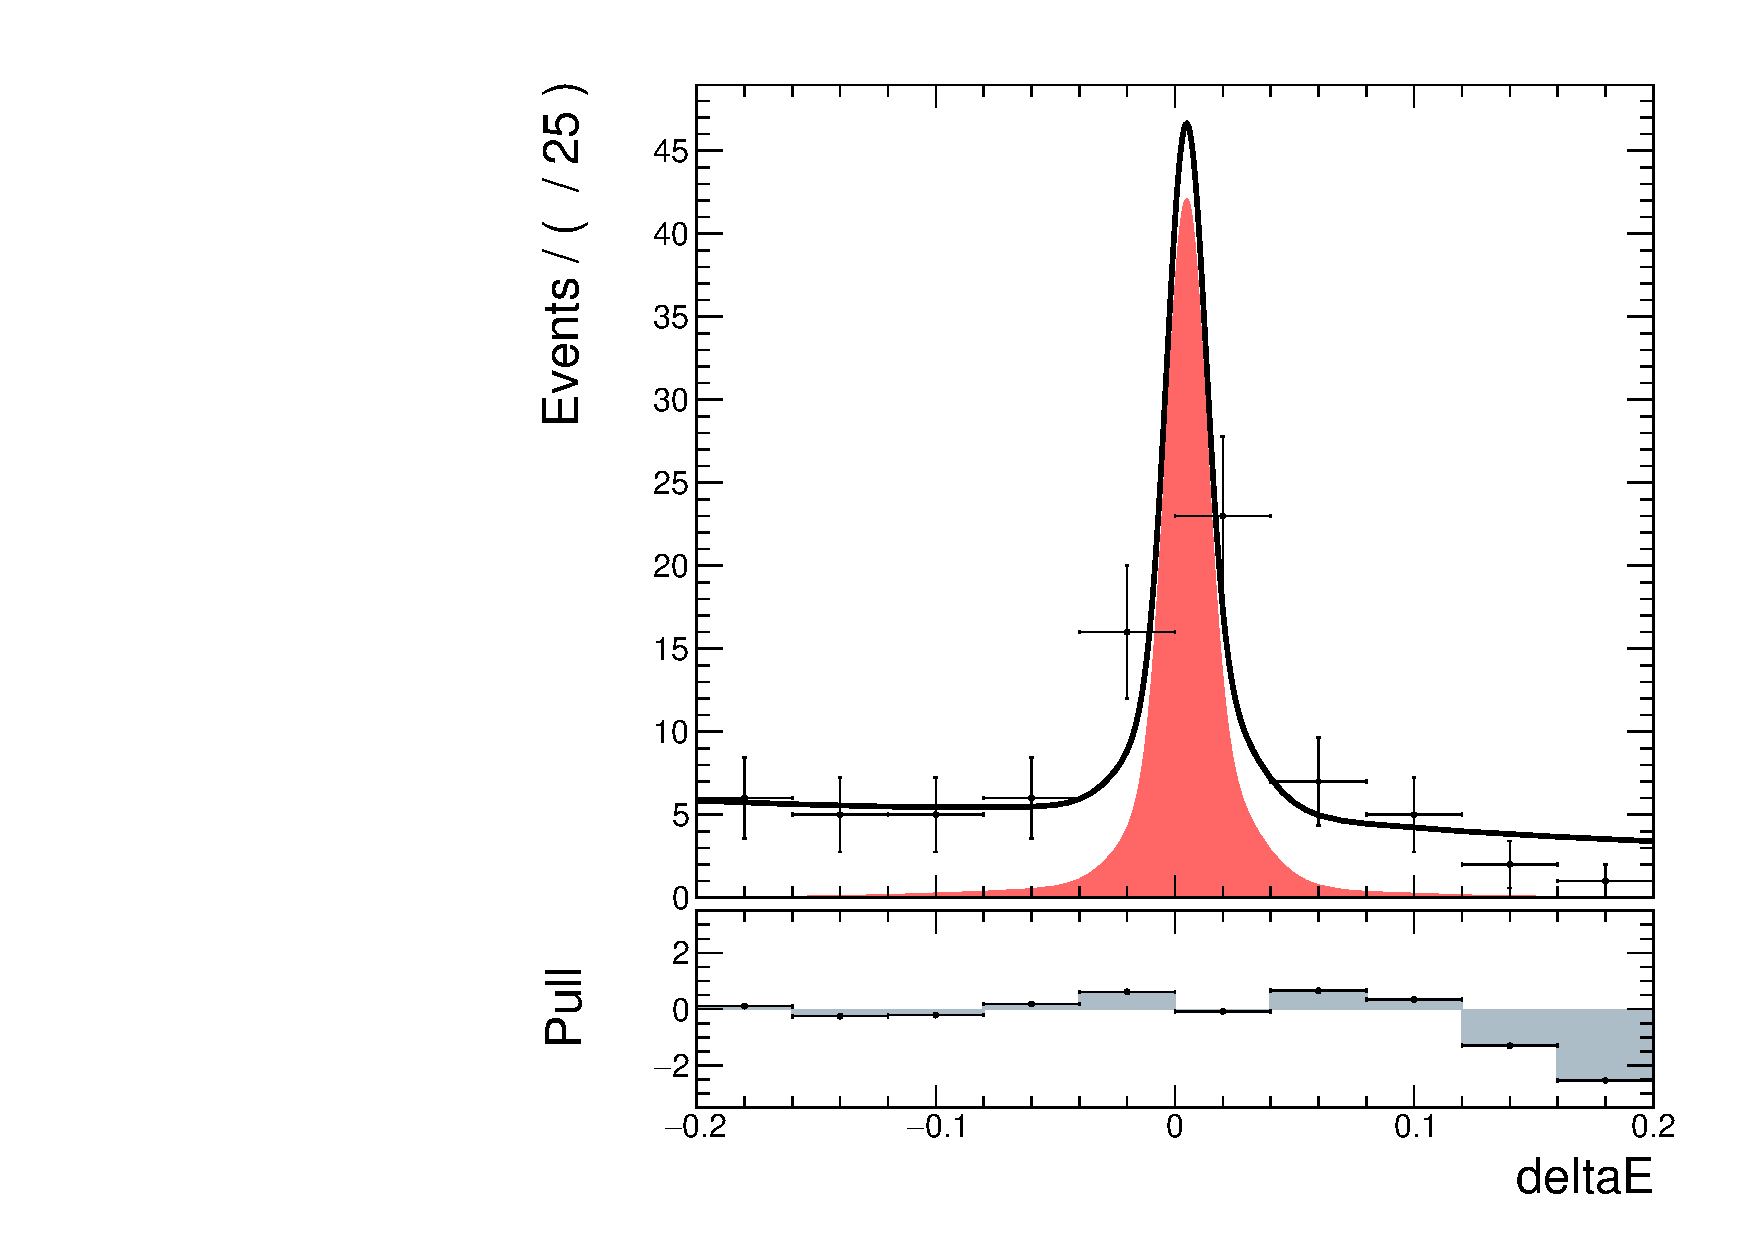
\includegraphics[page=1,height=5cm]{figures/injection_sig_30/ds_gen_deltaE_2D.pdf}
		\caption{signal injected: 30}
	\end{subfigure}
\caption{The fit results of $M_{bc}$ and $\Delta E$ in signal injection test, where signal events from 5 to 30 with 5 per step are injected with 46 continuum events.}
\label{fig:2Dinject}
\end{figure}


\begin{figure}[H]
	\begin{minipage}[b]{0.5\linewidth}
		\centering 
		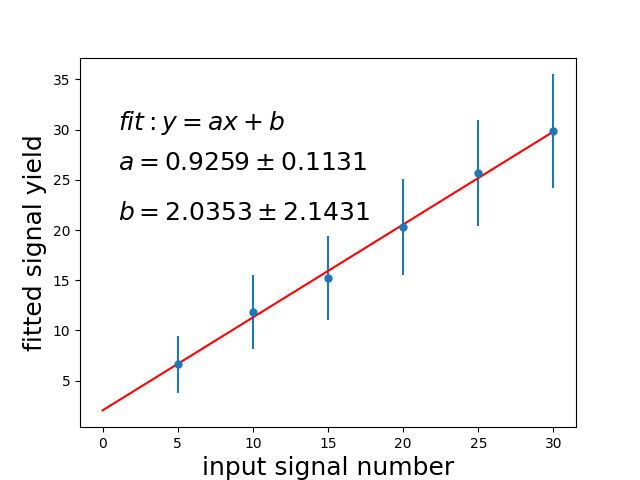
\includegraphics[height=5cm]{figures/inject_line_sig}
		\label{}
	\end{minipage}
	\begin{minipage}[b]{0.5\linewidth}
		\centering 
		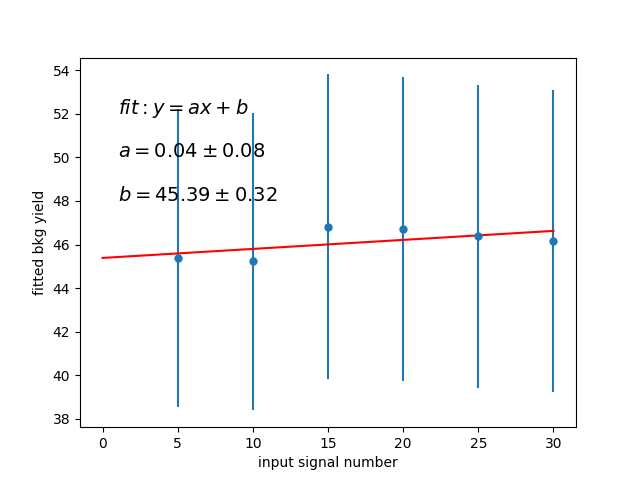
\includegraphics[height=5.2cm]{figures/inject_line_bkg}
		\label{}
	\end{minipage}
	\caption{Injection test for signal extraction. The linearity is clear between input and output signal events number.}
	\label{fig:2Dinjectline}
\end{figure}

\begin{comment}
\begin{figure}[htpb]
\centering 
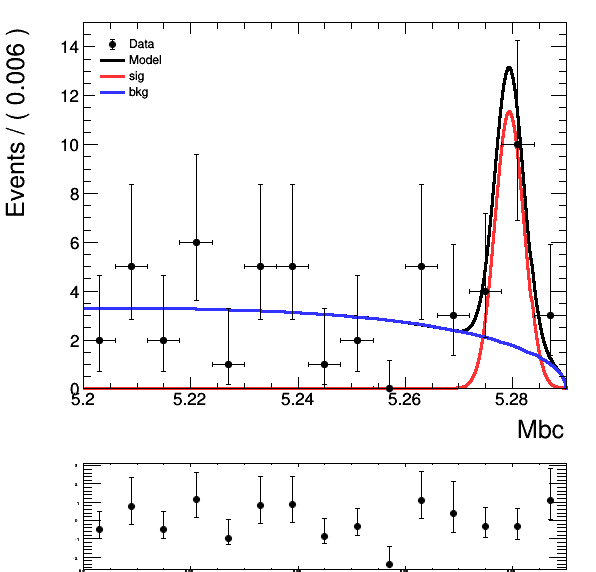
\includegraphics[width=0.7\linewidth]{data-mbc-fit}
\caption{$M_{bc}$ fit in data, signal is Gaussian and background is Argus.}
\end{figure}
\begin{figure}[htpb]
\centering 
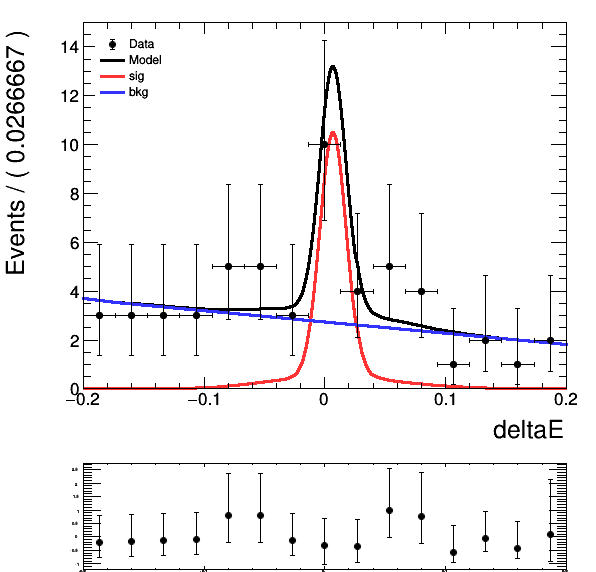
\includegraphics[width=0.7\linewidth]{data-dE-fit}
\caption{$\Delta{E}$ fit in data, signal is double-Gaussian and background is Chebyshev polynomial.}
\end{figure}
\begin{table}[htpb]
\centering
\caption{Fit results from RooFit on $M_{bc}$ and $\Delta E$}
\begin{tabular}{|c|c|c|}
\hline
Floating Parameters  & Mean Value & +/- Error  \\
\hline
N\_sig & 12.8 & 3.93\\
\hline
N\_bkg  & 41.2 & 6.62 \\
\hline
a0 & -0.34 & 0.264\\
\hline
$\chi_{argus}$ & -15.0 & 16.7\\
\hline
\end{tabular}
\end{table}

The fraction of signal and background can be obtained by integral over signal box region using 2D P.D.F. We define signal box using signal MC distribution in Fig 4.13 and 4.14, which $5.269 < M_{bc} < 5.287$ GeV and $-0.09 < \Delta E < 0.12$ GeV. The results are: 

\begin{eqnarray}
N_{sigbox} = 12.6 \pm 3.9\\
N_{bkgbox} = 2.6 \pm 0.2 
\end{eqnarray}

Compared with Belle experience, which similar analysis is done by using about 1$ab^{-1}$ data, signal yield is $327.1 \pm 19.4$. The estimated branching fraction of $B^0 \to K_S^0  K_S^0  K_S^0$ is: 
\end{comment}


\subsection{Kinematics and Vertexing Dependence on KsFinder} 

KsFinder largely reduce the combinatorial background of $B^0$ by improving $K_S^0$ purity. The previous section shows a good reconstruction performance at low statistics in early phase 3 data. Without the power of rejection provided by $K_S^0$ finder, rediscovery of $B^0 \to K_S^0  K_S^0  K_S^0$ in early phase 3 of Belle II won't be feasible. 
\begin{comment}
\begin{figure}[htpb]
\centering
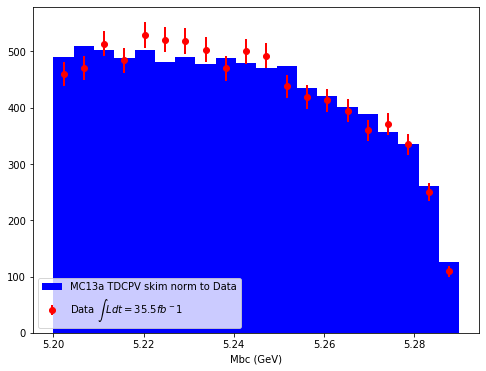
\includegraphics[width=0.7\linewidth]{mbc-noks}
\caption{$M_{bc}$ distribution in data(red) and MC(blue) without $K_S^0$ finder}
\end{figure}
\begin{figure}[htpb]
\centering
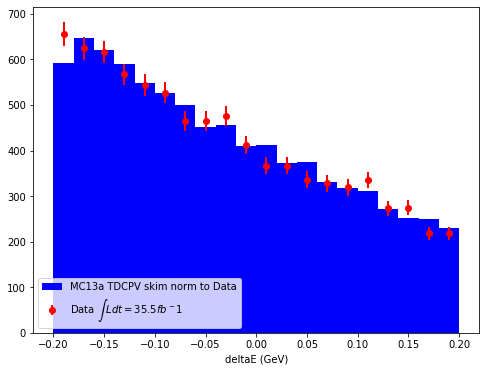
\includegraphics[width=0.7\linewidth]{dE-noks}
\caption{$\Delta{E}$ distribution in data(red) and MC(blue) without $K_S^0$ finder}
\end{figure}
\end{comment}

 However, it's essential to check the potential impact on kinematics and vertex positions of $B^0$ regarding the implementation of KsFinder. The $K_S^0$ classification uses information such as invariant mass and decay vertex positions which may propagate bias into $B^0$ kinematics and vertex information, eventually may affect the measuremnet of $\it{CP}$ parameters. Considering that 4 different types of $K_S^0$ based on their SVD hit numbers are used in $B^0$ reconstruction, the estimation with $B^0$ based on different $K_S^0$ types are required as well.
 
 Given each type of $B^0$ based on how many CDC-only tracks (meaning $B^0$ daughter $K_S^0$ are \textit{SVD00} type) it has in final states, the comparison on $M_{bc}$ and $\Delta{E}$ with or without KsFinder is done by fitting the distribution in signal MC. $M_{bc}$ and $\Delta{E}$ are both modeled by double Gaussian. The main Gaussian (with larger fraction) among the double Gaussian is used for checking the fit shape change by using KsFinder. Comparing corresponding fit results, no clear bias on $M_{bc}$ and $\Delta{E}$ is found by using KsFinder where the main Gaussian fit results are agreed well. The fit results are shown in Figure \ref{fig:mbc_bias} and \ref{fig:de_bias}. 
 
 \begin{figure}[htpb]
 	\centering
 	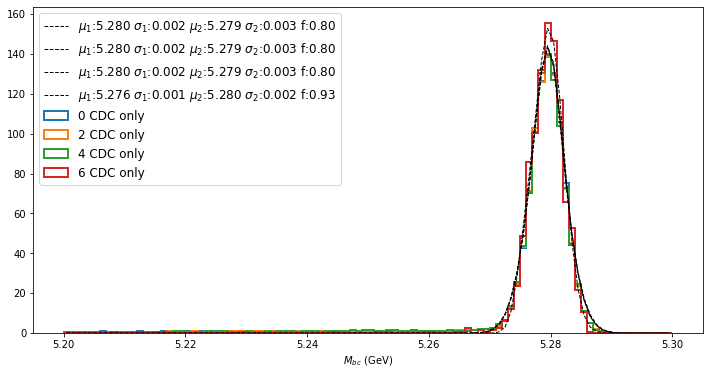
\includegraphics[width=0.7\linewidth]{bias-mbc}
 	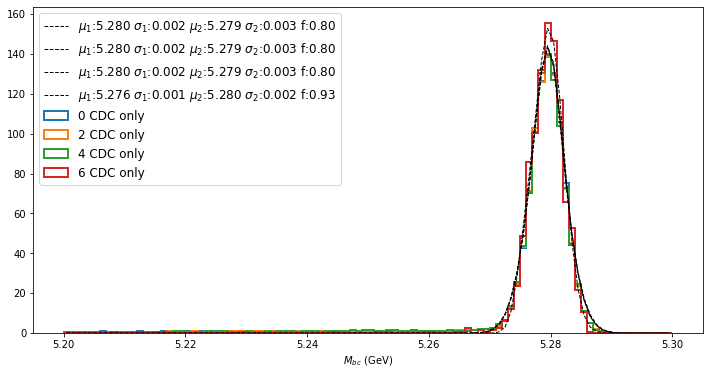
\includegraphics[width=0.7\linewidth]{bias-mbc-ks}
 	\caption{$M_{bc}$ distribution based number of CDC-only tracks in final states. Top: no KsFinder; Bottom: $K_S^0$ finder used.}
 	\label{fig:mbc_bias}
 \end{figure}
 \begin{figure}[htpb]
	\centering
	\includegraphics[width=0.7\linewidth]{bias-de}
	\includegraphics[width=0.7\linewidth]{bias-de-ks}
	\caption{$\Delta{E}$ distribution based number of CDC-only tracks in final states. Top: no KsFinder; Bottom: KsFinder used.}
	\label{fig:de_bias}
\end{figure}

Similar to the comparison of $M_{bc}$ and $\Delta{E}$, the Z direction vertex position and its uncertainties are also checked. No clear bias on vertex position and uncertainties are spotted either. The results are shown in Figure \ref{fig:bias-z} and \ref{fig:bias-zerr}. It obvious that the resolution of vertex on z-axis is much worse when the final states of $B^0$ only have CDC tracks. 

\begin{figure}[htpb]
	\centering
	\includegraphics[width=0.7\linewidth]{bias-z}
	\includegraphics[width=0.7\linewidth]{bias-z-ks}
	\caption{$\Delta z$ distribution based number of CDC-only tracks in final states. Top: no KsFinder; Bottom: KsFinder used.}
	\label{fig:bias-z}
\end{figure}
\begin{figure}[htpb]
	\centering
	\includegraphics[width=0.7\linewidth]{bias-zerr}
	\includegraphics[width=0.7\linewidth]{bias-zerr-ks}
	\caption{$\delta\Delta z$ distribution based number of CDC-only tracks in final states. Top: no KsFinder; Bottom: KsFinder used.}
	\label{fig:bias-zerr}
\end{figure}
Above all, no strong appearance of bias on kinematics and vertex positions from using KsFinder has been found, KsFinder may implement a small shift on the vertex position which is neglect-able  compared to the large statistical uncertainty due to low luminosity. For the moment, there's no correction on these observables are applied.
